\documentclass[8pt]{beamer}

\usetheme{Singapore}
\usefonttheme{serif} 


%%%%%%%%%%%%%%%%%%%%%%%%
% Usual LaTeX Packages %
%%%%%%%%%%%%%%%%%%%%%%%%
\usepackage{pdfpages}
\usepackage{amsmath}
\usepackage{amscd}
\usepackage{amsfonts}
\usepackage{amssymb}
\usepackage{graphicx}
\usepackage{mathrsfs} 			% For Weinberg-esque letters
\usepackage{cancel}				% For "SUSY-breaking" symbol
\usepackage{slashed}            % for slashed characters in math mode
\usepackage{bbm}                % for \mathbbm{1} (unit matrix)
\usepackage{dsfont}
\usepackage{amsthm}				% For theorem environment
\usepackage{multirow}			% For multi row cells in table
\usepackage{arydshln} 			% For dashed lines in arrays and tables
\usepackage{multirow}
\usepackage{multicol}
\usepackage{bigstrut}
\usepackage{setspace}
\usepackage{endnotes}
\usepackage{etex}
\usepackage{lmodern}
\usepackage{booktabs}
\usepackage{graphics}
\usepackage[flushleft]{threeparttable}
%\usepackage{enumitem}
%\setlist[itemize]{itemsep=2mm}
\usepackage{array}
\usepackage{color}
\usepackage{colortbl}
\usepackage{hyperref}
\usepackage{ifplatform}
\usepackage{dcolumn}
\usepackage{threeparttable}
\usepackage{hyperref}
\usepackage{tabularx}
\usepackage{soul}
\usepackage{ulem}

\usepackage[utf8]{inputenc}
\usepackage[T1]{fontenc}
\usepackage{appendixnumberbeamer}
\usepackage{xcolor}
\def\boxit#1{%
  \smash{\color{red}\fboxrule=1pt\relax\fboxsep=2pt\relax%
  \llap{\rlap{\fbox{\vphantom{0}\makebox[#1]{}}}~}}\ignorespaces
}
\usepackage{appendixnumberbeamer}

\newcommand{\E}{\mathbb{E}}

% Code for Hiding Columns in Tables
\newcolumntype{H}{>{\setbox0=\hbox\bgroup}c<{\egroup}@{}}


\graphicspath{{images/}}	% Put all images in this directory. Avoids clutter.





% BIBLIOGRAPHY (OPTION: BIBLATEX) ===========================================
\usepackage{csquotes}
\usepackage[natbib = true, backend = biber, style  = authoryear-icomp]{biblatex}
\addbibresource{References.bib}

\usepackage{setspace}
\setbeamercovered{transparent}

%gets rid of navigation symbols
\setbeamertemplate{navigation symbols}{}

\setbeameroption{show notes}
%\setbeameroption{show only notes}
%\setbeameroption{hide notes}

% A simple slide counter at the bottom of the slide
\setbeamertemplate{footline}{
   \begin{beamercolorbox}[ht=4ex,leftskip=0.3cm,rightskip=0.3cm]{author in head/foot}
    \vspace{0.1cm}
    \hfill \insertframenumber / \inserttotalframenumber
  \end{beamercolorbox}
   \vspace*{0.1cm}
} 

\newcommand\independent{\protect\mathpalette{\protect\independenT}{\perp}}
\def\independenT#1#2{\mathrel{\rlap{$#1#2$}\mkern2mu{#1#2}}}

\setbeamercovered{transparent}


\title{The limits of self-commitment and private paternalism \\
Preliminary --comments welcome}
\author{Craig McIntosh \and Isaac Meza \and Joyce Sadka \and Enrique Seira \and Francis J.\ DiTraglia }

\date{February 2023}

%\setbeamercolor{section in head/foot}{bg=darkcrimsonred}
\setbeamersize{text margin left=11pt, text margin right=11pt}
%\setbeamertemplate{section in toc}[square]




%%%%%%%%%%%%%%%%%%%%%%%%%%%%%%%%%%%%%%%
%%%%%%%%%%%%%%%%%%%%%%%%%%%%%%%%%%%%%%

\begin{document}


\begin{frame}[c, noframenumbering]%{\phantom{title page}}
% The \phantom{title page} is a kludge to get the red bar on top
\titlepage
\end{frame}


\section{Motivation}



\begin{frame}{Motivation: Private paternalism}
\begin{itemize}
    \vfill \item Many institutions —firms, schools, financial contracts— restrict choice using built-in commitment mechanisms which help workers, students, borrowers overcome self-control problems
    \begin{itemize}
        \item Loans with fixed repayment schemes, homework due dates, etc.
    \end{itemize}
    \vfill\item At the same time these firms hide these forcing mechanisms and don’t market their commitment features, potentially because demand for them is low.
    \vfill \item  Laibson (2018) argues that clients that benefit from commitment may underestimate its value, and that in such cases private paternalism could be beneficial.
    \vfill \item  We study the benefits of imposing a fixed payment structure in loans, whether there is demand for it, and whether non-takers of such a commitment product would benefit from taking it.
\end{itemize}

\end{frame}


\begin{frame}{Context}
\begin{itemize}
    \vfill \item Pawn loans involve borrowers leaving valuable liquid assets as collateral in exchange for an immediate cash loan
    \vfill \item Because the loan is overcollateralized and collateral is liquid, the lender approve loans in a few minutes without income or credit history check $\rightarrow$ used for emergencies.
    \vfill \item This may explain why they are highly popular: $>$11,000 pawn shops across the US, with 30 million clients and \$14 billion yearly revenues.
    \begin{itemize}
        \item Our partner pawn lender alone approved 4 million loans in \hl{2017-2020}.
        \item Pawn lending has existed at least since the Roman empire.
    \end{itemize} 
    \vfill \item Controversial: interest rates and default rates are high, and used by people in distress.
    \vfill \item Regulators believe mostly unsophisticated borrowers use it.
\end{itemize}
\end{frame}




\begin{frame}{Methodological Contribution}
\begin{itemize}
    \vfill \item How do treatment effects relate to selection?  Key question in many literatures:
	\begin{itemize} 
		\item HTEs, MTE, LATEs, what is learned from IV regressions (Heckman \& Vytlacil, 2005).
		\item Health effects of universal versus elective interventions
		\item Optimal targeting (Alatas et al. 2012)
	\end{itemize}
     \vfill \item A context of particular interest to behavioral literature:  the demand for commitment in financial contracts (Laibson 1997, Bryan et al. 2010).
     \vfill \item Key quantity in debate about paternalism:  impacts on those who wouldn't elect to take the program versus impacts on those that do.
     \vfill \item Three-arm design:  Control, Choice (voluntary takeup=ITT), Forcing (universal=ATE).  We illustrate how to use standard exclusion restrictions for point identification:
    \begin{itemize}
        \item Treatment on the Treated (ToT) and 
        \item Treatment on the Untreated (TUT), also (ToT-TUT)
	\item Average Selection Bias, and Average Selection on Levels
    \end{itemize} 
   \vfill   \item Consider winners and losers from paternalism using bounding, Random Forest estimation of individual treatment effects. 
\end{itemize}
\end{frame}


\begin{frame}{Our partner: logistics, contract, stats}
    \begin{itemize}
        \item Partnered with one of the largest pawn lender in Mexico (hundreds of branches)
        \vfill\item Logistics: 
        \begin{itemize}
            \vfill\item Appraising:  gold jewelry as collateral the appraiser tests and weights the gold and assesses its value (5 mins).
           \vfill \item Loan: if the borrower agrees to leave the piece the appraiser gives 70\% of the gold value in cash, no checking of credit history or income.
           \vfill \item Contract (Standard in industry): 
           \begin{itemize}
               \vfill\item Interest rate = 7\% \textit{per month} compounded daily on the outstanding amount. No reminders.
               \vfill\item To recover pawn need to pay principal plus the accumulated interest. If this does not happen, pawnbroker keeps the piece and any payments made.
               \vfill\item  Client can renew for 3 months paying the accumulated interest and signing a new contract.
           \end{itemize}
        \end{itemize}

    \end{itemize}
\end{frame}




\begin{frame}{Context}
\begin{columns}
\begin{column}{.45\textwidth}

\begin{figure}[H]
    \begin{center}
    \caption{Pawnshop}
        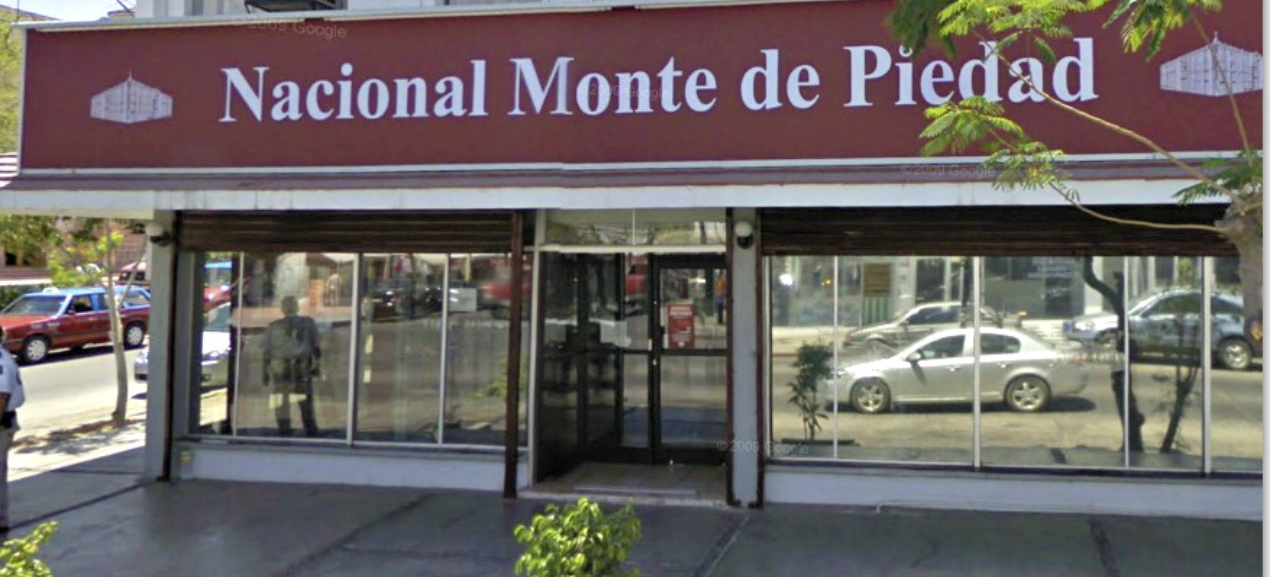
\includegraphics[width=0.95\textwidth]{Figuras/empenio2.png}
    \end{center}
    \end{figure}
\begin{figure}[H]
    \begin{center}
    \caption{Appraiser/tellers inside a pawnshop}
        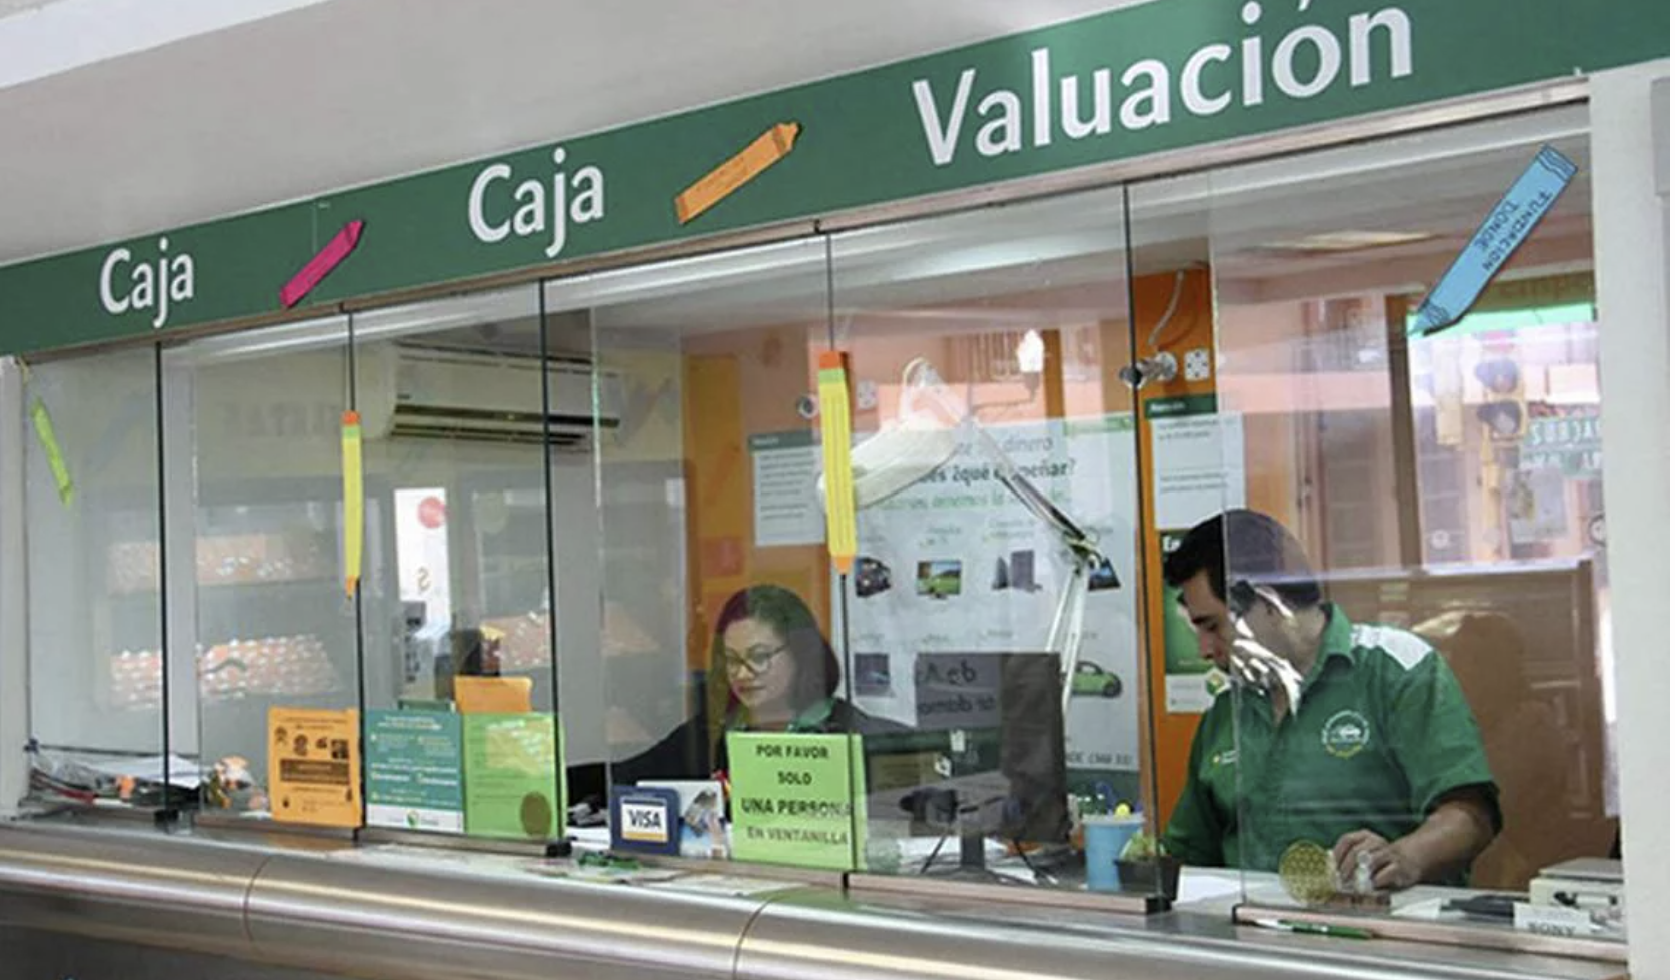
\includegraphics[width=0.95\textwidth]{Figuras/empenio9.png}
    \end{center}
    \end{figure}    
    
    \end{column}
    
\begin{column}{.45\textwidth}

\begin{figure}[H]
    \begin{center}
    \caption{Pawnshop}
        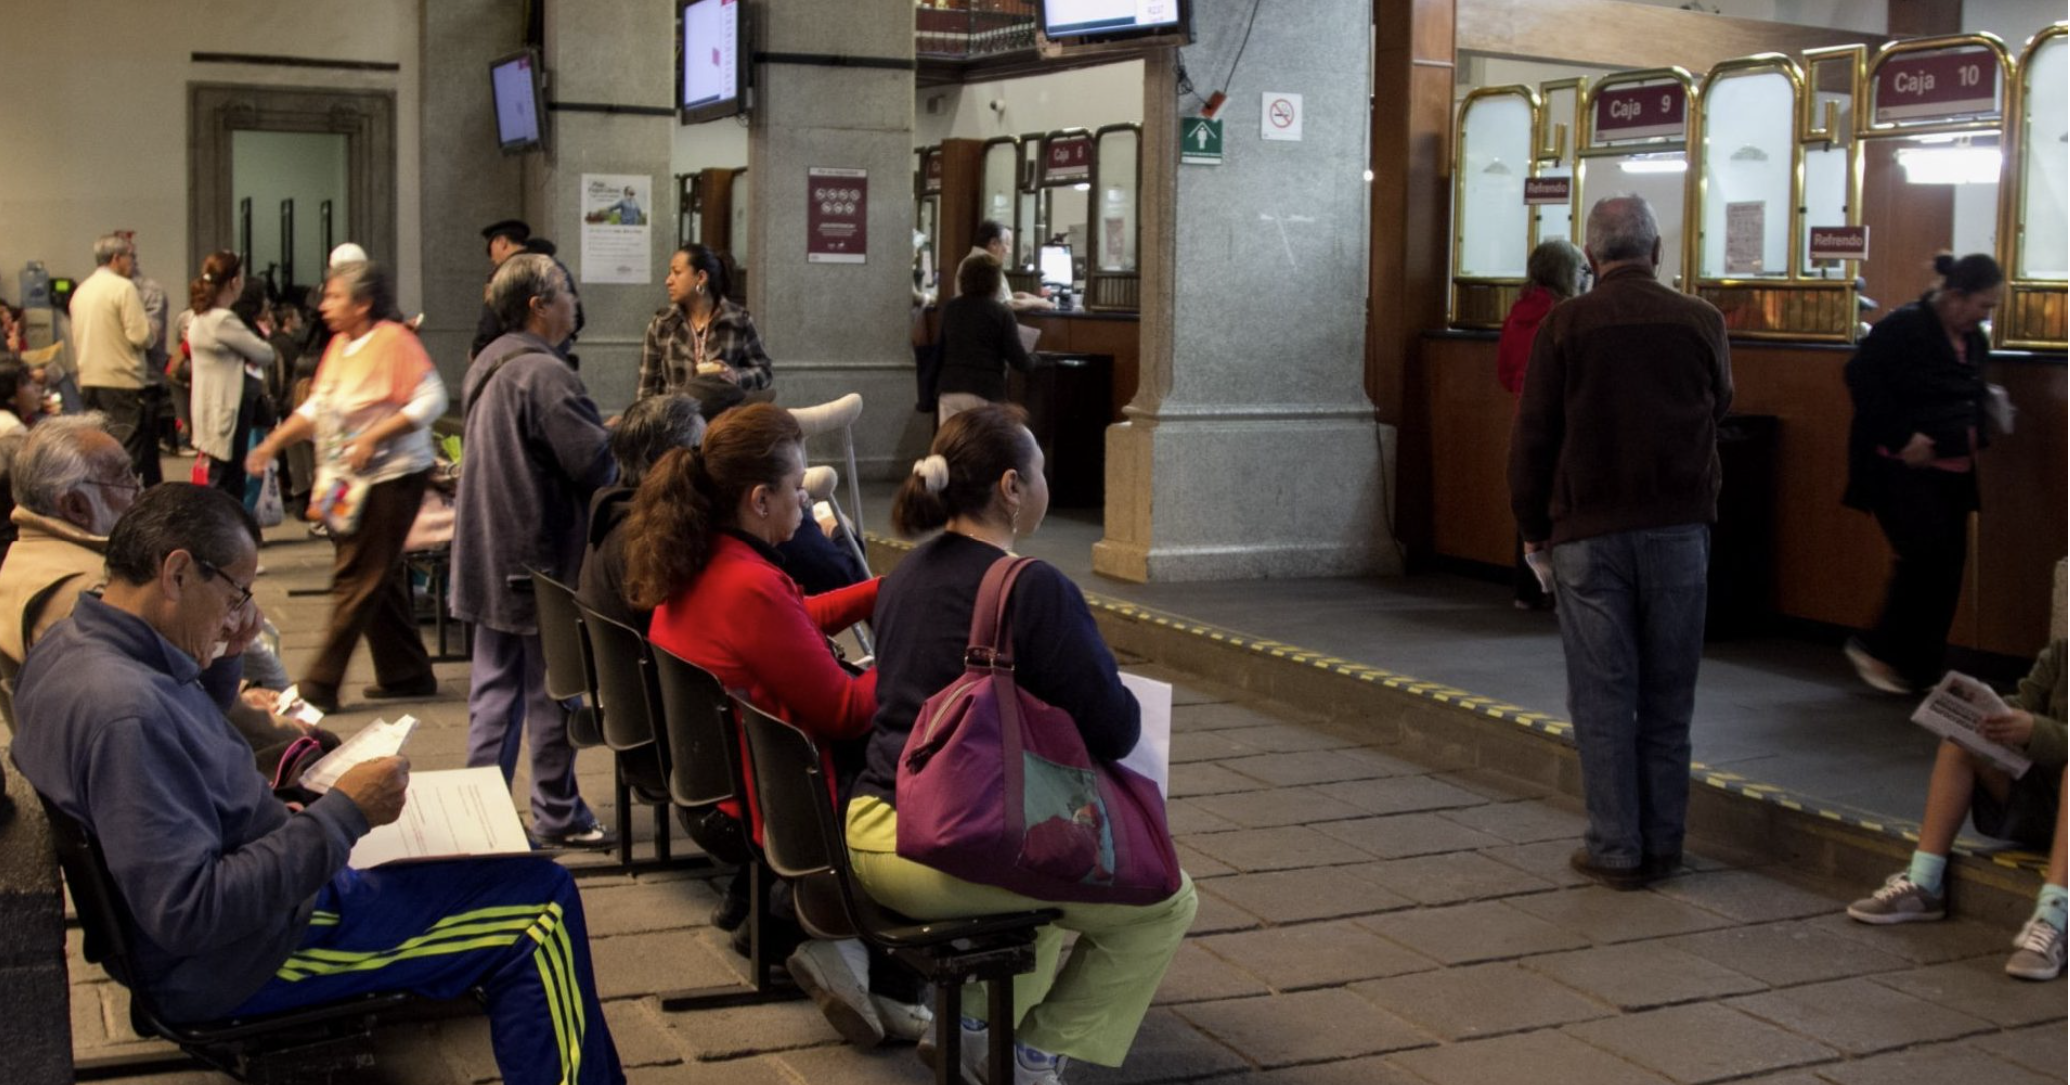
\includegraphics[width=0.95\textwidth]{Figuras/empenio11.png}
    \end{center}
    \end{figure}
\begin{figure}[H]
    \begin{center}
    \caption{Lost pawns which are for sale}
        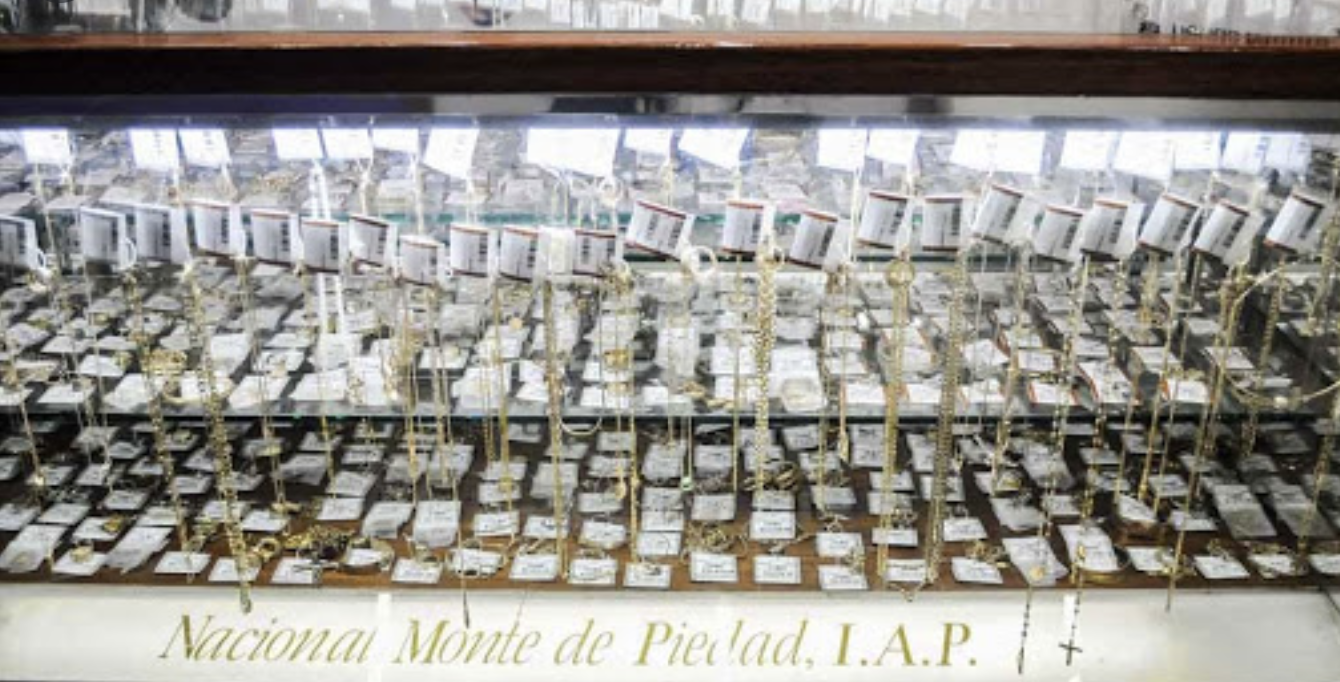
\includegraphics[width=0.95\textwidth]{Figuras/empenio3.png}
    \end{center}
    \end{figure}    
    
    \end{column}    
    \end{columns}
\end{frame}




\begin{frame}{Lenders incentives}
    \begin{itemize}
        \item Because the loan is overcollateralized and collateral is liquid, the lender may gain if the borrower defaults on the loan, especially if the borrower pays towards recovery on the way to default.
        \item In fact, 60\% of clients lose their pawn in a time span of 230 days.
        \item Among those that lose their pawn, 48\% paid a positive amount towards its recovery and on average paid 42\% of loan.
        \item This happens in spite (or because?) of 74\% of borrowers reporting a 100\% subjective probability recovery ex-ante. 
        \item XXX of borrowers are classified as present biased using the simple standard question.
        \item In such an environment, one may ask if putting more structure in payments may help borrowers recover their pawn.
        \item We may particularly care about this if borrowers are vulnerable: 30\% of them could not pay either water, electricity \& gas or rent in the past 6 months; 87\% said they are pawning because of an emergency.
    \end{itemize}
\end{frame}



\begin{frame}{Structured payments contract}
   \begin{itemize}
       \vfill \item We designed a new contract that is identical to the status quo contract except that it enhances the regularity and salience of payments as a way to encourage repayment.
       \vfill\item The contract requires 3 equal payments in the 30th, 60th, ad 90th days of the loan, with the imposition of a 2\% fee of the amount owed if the client fails to pay.
       \vfill\item The propose of the small fee was to mainly to make the structured schedule salient, not to be a large disincentive to be late. 
       \begin{itemize}
           \item Transportation cost to go to the branch to pay is on the same order of magnitude as the fee in average.
       \end{itemize}
       \vfill\item  The empirical literature provides some guidance that such a contract may decrease default and elicit demand.
       \begin{itemize}
           \item Field \& Pande (2008) find null effects of payment frequency on loan default for group lending (but samples are small and there almost no default in the control). 
           \item XXX CITE PAPERS where frequency helps
        \item  Bauer et al. (2012) estimate a positive correlation between measured present bias and and selecting into microfinance, which they interpret demand for structured payments.
       \end{itemize}
       
   \end{itemize}
    
\end{frame}


\section{Measures}

\begin{frame}{Data}
\begin{itemize}
    \item Administrative data: XX months before and XX months after the experiment ended
    \begin{itemize}
        \item Unique identifier for each client and for the piece.
        \item Value of the item, money loaned (70\%), date of pawning
        \item For all payments: date and amounts
        \item Fees incurred
        \item Whether the client lost the pawn, renewed the contract
    \end{itemize} 

    \vfill \item Survey data
    \begin{itemize}
        \item During experiment, we asked clients to complete a 5-minute survey before going to the teller window to appraise their piece and before treatment status was known to them.
        \item Demographics, proxies for income/wealth, education, present-biased preferences, experience pawning, if family or friends commonly asked for money, cost of going to branch, the subjective probability of recovering, the subjective value, etc.
    \end{itemize}
\end{itemize}    
\end{frame}


\begin{frame}{Main outcomes: financial cost and default}

\begin{itemize}
    \item We are interested in measuring the financial cost of borrowing, which very saliently includes the cost of defaulting on the loan and losing the pawn.
    \item We will measure loan default using an indicator $\mathds{1}(\text{Default}_i)$, and the cost in pesos using the following definition that capture borrower outlays:
\end{itemize}

   \begin{equation*}
    \text{Financial Cost}_i =  \underbrace{\sum_t P^i_{it}}_{\text{Pay to Interest}} + \underbrace{\sum_t P^f_{it}}_{\text{Pay to Fees}}  + \mathds{1}(\text{Default}_i) \times \left[\text{Pawn Val}_i + \underbrace{\sum_t P^c_{it}}_{\text{Pay to Capital}} \right]
   \end{equation*}

\begin{itemize}
    \vfill \item Towards the end of the presentation we will show results that apply a time discount factor.

\end{itemize}
\end{frame}


\begin{frame}{Distribution of financial cost (\$MXN)}
    \begin{figure}
     \centering
        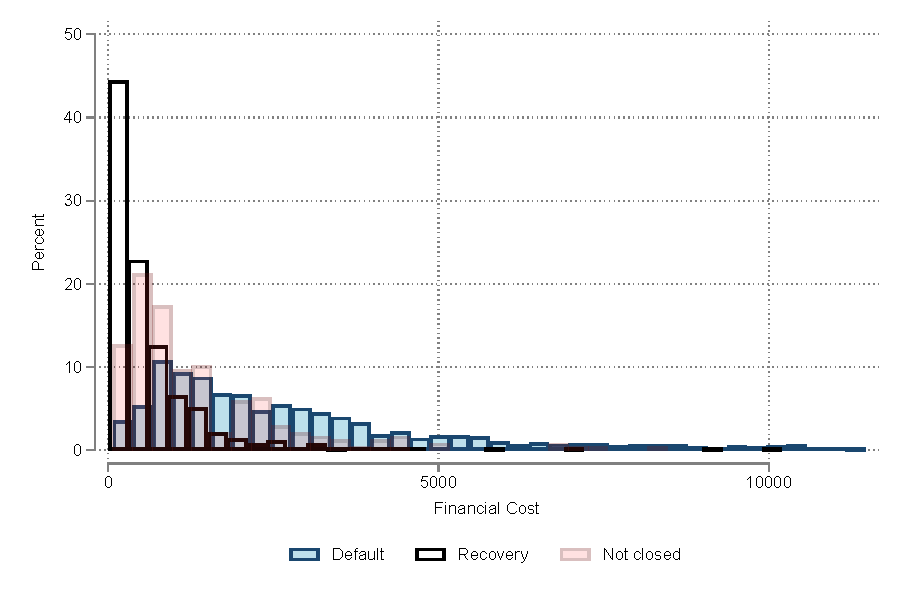
\includegraphics[width=.8\textwidth]{Figuras/hist_fc.pdf}
    \end{figure}
\end{frame}


\begin{frame}{Distribution of APR}
\vspace{.2in}
\begin{equation*}
    (\text{APR})_i =\left( 1 + \frac{\frac{\text{Financial Cost}_i}{\text{Appraised Value}_i}}{\text{loan term}_i}\right)^{\text{loan term}_i}-1
\end{equation*}
\vspace{.2in}
\begin{figure}
     \centering
        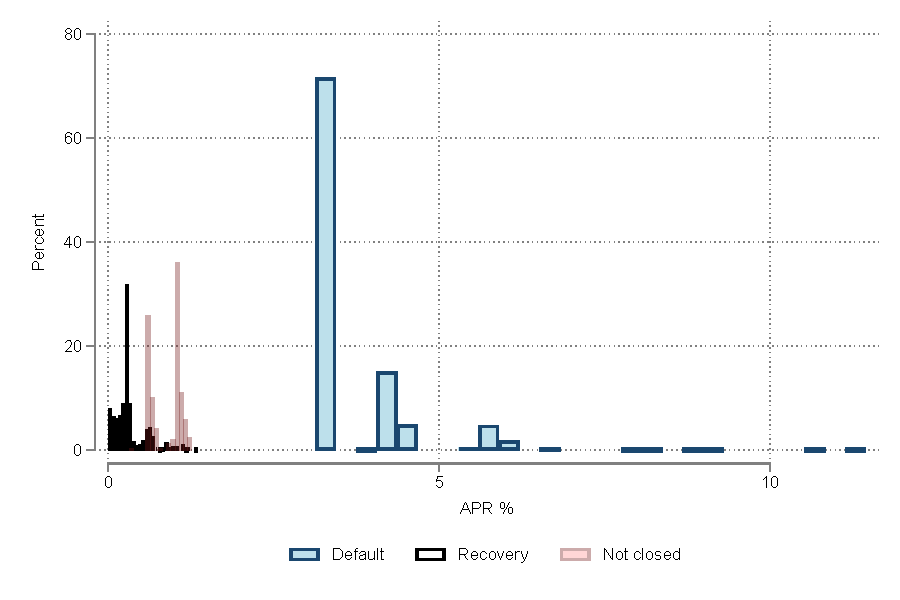
\includegraphics[width=.75\textwidth]{Figuras/hist_apr.pdf}
    \end{figure}
\end{frame}

    
%\begin{frame}{Measuring Borrowers Financial Cost}
%\begin{columns}
%\begin{column}{.5\textwidth}
%    \begin{figure}[H]
%     \caption{Financial cost (MXN)}
%    \begin{center}
%    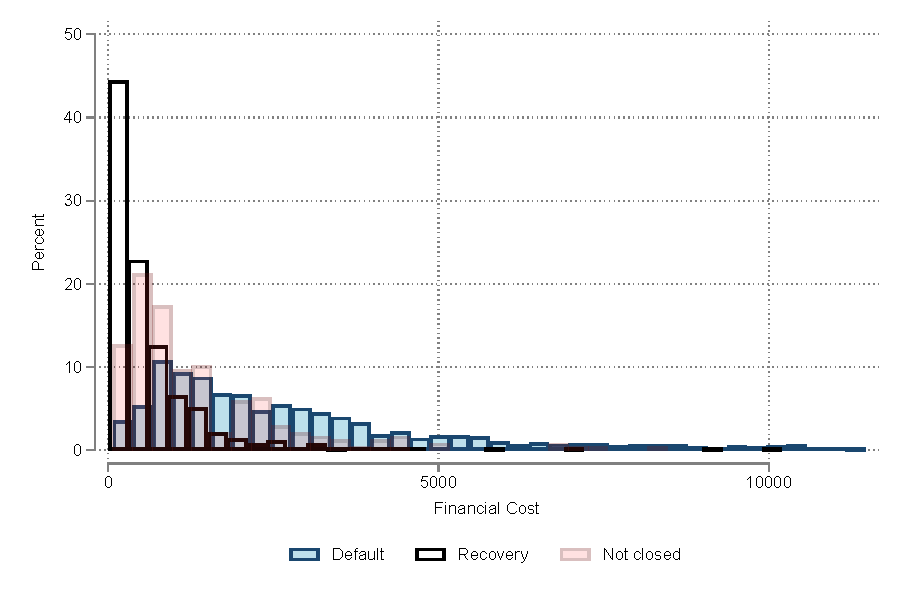
\includegraphics[width=\textwidth]{Figuras/hist_fc.pdf}
%    \end{center}
%    \end{figure}
%    \resizebox{1.0\linewidth}{!}{
%  \begin{minipage}{\linewidth}
%    \tiny{
    %\begin{align*}
    %\text{Financial Cost}_i =&  \underbrace{\sum_t P^i_{it}}_{\text{Pymnts to interests}} + \underbrace{\sum_t P^f_{it}}_{\text{Pymnts of fees}} \\
  %& + \underbrace{\mathds{1}(\text{Default}_i) \times (\text{Appraised Value}_i}_{\text{Cost of losing pawn}} + \underbrace{\sum_t P^c_{it}}_{\text{Pymnts to capital}})
%\end{align*}
%}
%  \end{minipage}
%}

%\end{column}
%\begin{column}{.5\textwidth}
%    \begin{figure}[H]
%     \caption{Effective APR}
%    \begin{center}
%    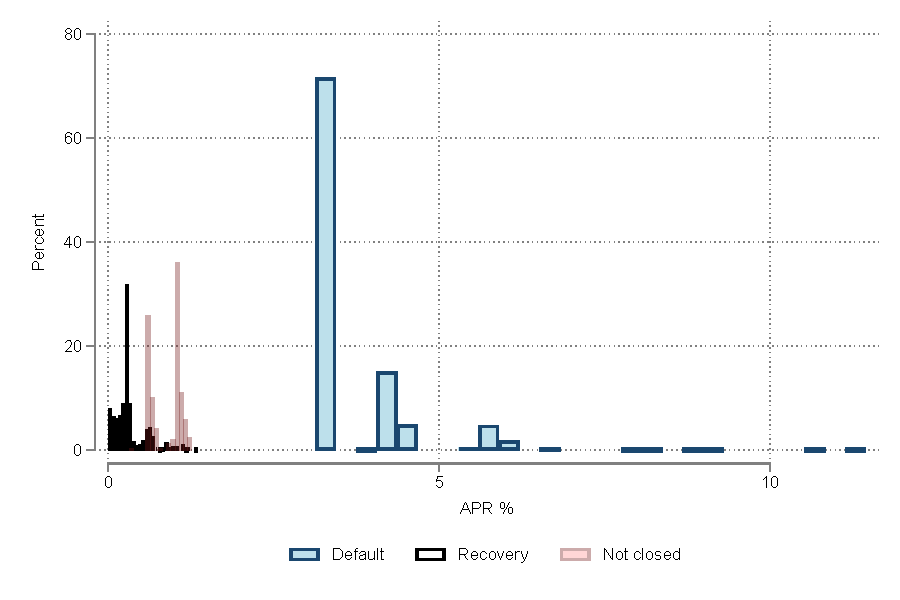
\includegraphics[width=\textwidth]{Figuras/hist_apr.pdf}
%    \end{center}
%    \end{figure}
%    \resizebox{.95\linewidth}{!}{
%  \begin{minipage}{\linewidth}    
%    \tiny{
    %\begin{align*}
    %(\text{APR})_i =&\left( 1 + \frac{\frac{\text{Financial Cost}_i}{\text{Appraised Value}_i}}{\text{loan term}_i}\right)^{\text{loan term}_i}-1 \\
   % & \\
   % & \\
   % & \\
   % &
%\end{align*}
%}
 % \end{minipage}
%}
%\end{column}
%\end{columns}
%\end{frame}



\section{Design}



\begin{frame}{Treatment arms}
   \begin{itemize}
    \vfill \item Randomization at the branch-day level. 
    \begin{itemize}
        \vfill \item Control arm 
       \vfill \item Forced Commitment arm
       \vfill \item Choice Commitment arm
    \end{itemize}
    \vfill \item The  existence  of  a  choice  arm  allows  us  not  only  to  measure  if  there  is  demand  for  such  a contract, but who demands it, not only in demographic terms, but in terms of potential treatment effects.
   \vfill \item  This design is innovative and critical for our purposes, as it enables us to explore whether or not forcing people into a structured payment contract could be more beneficial than allowing choice for a significant fraction of them
\end{itemize}
\end{frame}


\begin{frame}{Description}

\begin{figure}[H]
     \caption{Experiment description}
    \label{exp_description}
\begin{center}
        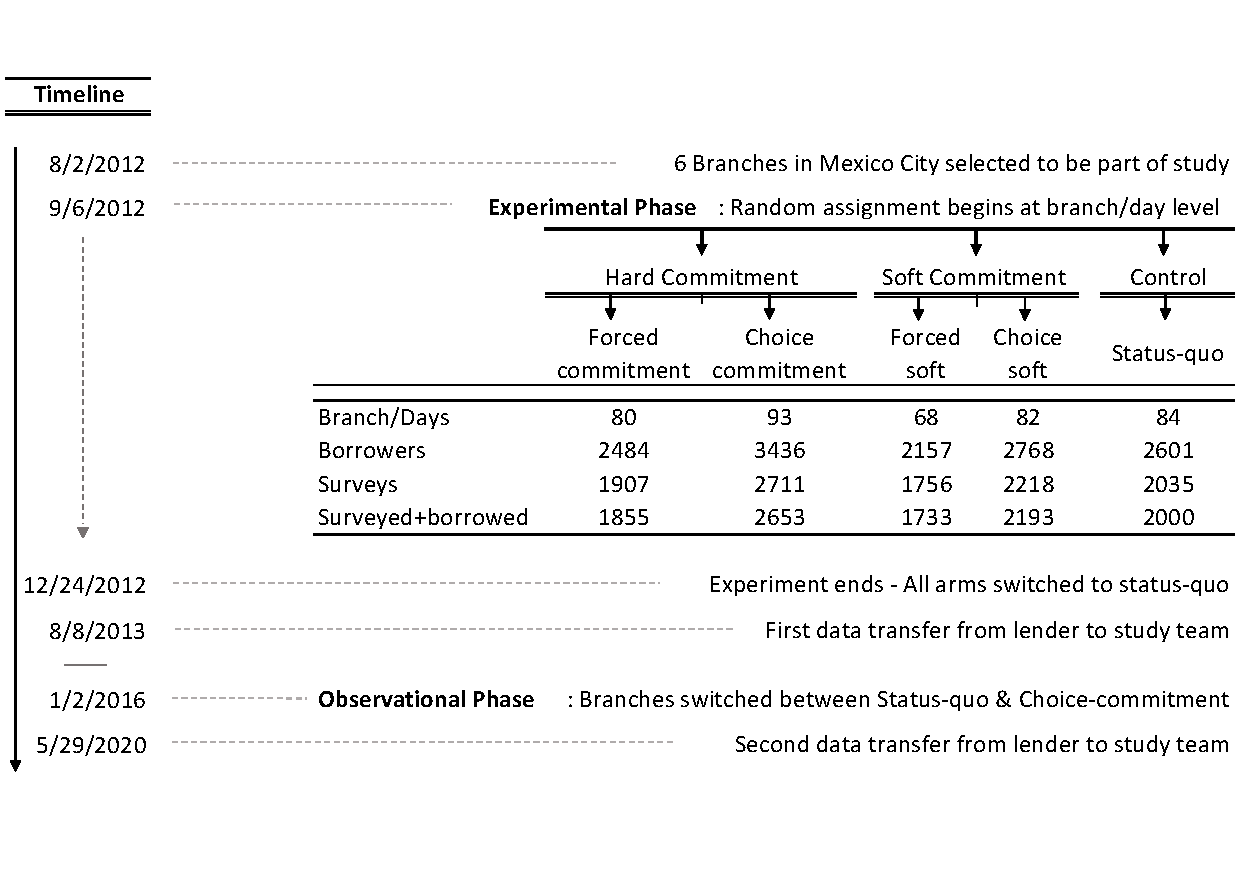
\includegraphics[width=0.85\textwidth]{Figuras/consort.pdf}
  \end{center}
\end{figure}

\end{frame}


\begin{frame}{Experimental integrity}
    \begin{table}[H]
\caption{Attrition table}
\label{attrition_table}
\begin{center}
\scriptsize{% Table generated by Excel2LaTeX from sheet 'Attrition'
\begin{tabular}{lcccr}
\toprule
      & Control & Structure & Choice & \multicolumn{1}{c}{p-value} \\
\midrule
\midrule
Loan take-up & 0.967 & 0.955 & 0.961 & 0.82 \\
      & (0.01) & (0.01) & (0.01) &  \\
\midrule
Number of borrowers & 20.8  & 22.2  & 25.4  & 0.17 \\
      & (3.29) & (3.9) & (4.89) &  \\
\rowcolor[rgb]{ .949,  .949,  .949} \multicolumn{1}{r}{median} & 19    & 20    & 21    & 0.5 \\
\midrule
Number of pawns/borrower & 1.4   & 1.4   & 1.4   & 0.43 \\
      & (0.08) & (0.04) & (0.05) &  \\
\rowcolor[rgb]{ .949,  .949,  .949} \multicolumn{1}{r}{median} & 1.4   & 1.3   & 1.3   & 0.6 \\
\midrule
Number of pawns  & 31    & 31.3  & 37.2  & 0.24 \\
      & (5.8) & (5.6) & (7.9) &  \\
\rowcolor[rgb]{ .949,  .949,  .949} \multicolumn{1}{r}{median} & 27    & 28    & 30    & 0.46 \\
\midrule
Amt borrowed/borrower & 2266.8 & 2094  & 2115.2 & 0.18 \\
      & (101.8) & (83.7) & (99.9) &  \\
\rowcolor[rgb]{ .949,  .949,  .949} \multicolumn{1}{r}{median} & 2154.3 & 2041  & 2047.5 & 0.65 \\
\midrule
Total borrowed & 47877 & 47813 & 54780 & 0.4 \\
      & (8005) & (9436) & (12587) &  \\
\rowcolor[rgb]{ .949,  .949,  .949} \multicolumn{1}{r}{median} & 37520 & 39420 & 40850 & 0.73 \\
\midrule
Obs   & 85    & 81    & 94    &  \\
\bottomrule
\bottomrule
\end{tabular}%
}
\end{center}
\end{table}
\end{frame}


\begin{frame}{Balance}

\vfill ISAAC: can you put the balance table here?
    
\end{frame}


\section{Results}
\begin{frame}{Main results}
    
 \begin{equation*} \label{basic_reg}
    y_{ij} = \alpha + \beta^F T_{i}^F + \beta^C T_{i}^C + \gamma X_{ij} + \epsilon_{ij}
\end{equation*}

\begin{table}[H]
\caption{Main treatment effects}
\label{main_impact_table}
\begin{center}
\resizebox{0.95\textwidth}{!}{
\scriptsize{% Table generated by Excel2LaTeX from sheet 'decomposition_main_te_pres'
\begin{tabular}{lcccccccc}
\toprule
      &       & \multicolumn{5}{c}{Components of FC}  &       &  \\
\cmidrule{3-7}      & FC    & Int. pymnt & Fee pymnt & Princ. pymnt & Lost pawn val & Default &       & APR \\
\midrule
      & (1)   & (2)   & (3)   & (4)   & (5)   & (6)   &       & (7) \\
\midrule
\midrule
Forced cmit & -379.7*** & -157.3*** & 32.1*** & -0.57 & -254.5** & -0.065*** &       & -0.34*** \\
      & (111.4) & (34.9) & (1.43) & (3.03) & (104.8) & (0.023) &       & (0.080) \\
Choice cmit & -84.9 & -24.9 & 1.34** & -3.98 & -61.4 & -0.025 &       & -0.12 \\
      & (114.6) & (38.4) & (0.54) & (2.47) & (109.2) & (0.021) &       & (0.073) \\
      &       &       &       &       &       &       &       &  \\
\midrule
Observations & 6304  & 6304  & 6304  & 6304  & 6304  & 6304  &       & 6304 \\
R-squared & 0.007 & 0.022 & 0.151 & 0.003 & 0.007 & 0.013 &       & 0.011 \\
Control Mean & 1851.0 & 545.9 & 0     & 5.82  & 1305.1 & 0.44  &       & 1.84 \\
\bottomrule
\bottomrule
\end{tabular}%
}
}
\end{center}
%\textit{Do file: } \texttt{decomposition\_main\_te.do}
\end{table}
\end{frame}


\begin{frame}{Mechanisms}


\only<1>{
\begin{table}[H]
\caption{Intermediate outcomes}
\label{mechanisms}
\begin{center}
\resizebox{0.7\textwidth}{!}{
\scriptsize{% Table generated by Excel2LaTeX from sheet 'mechanism_pres'
\begin{tabular}{lcc}
\toprule
      & \multicolumn{2}{c}{Panel A  : Speed of payment} \\
\cmidrule{2-3}      & Days to 1st payment & \% of payment in 1st visit \\
\midrule
\midrule
      & (1)   & (2) \\
\midrule
\midrule
Forced cmit & -13.8*** & 7.70*** \\
      & (1.61) & (2.78) \\
Choice cmit & -3.51** & -0.85 \\
      & (1.57) & (2.19) \\
      &       &  \\
\midrule
Observations & 4412  & 6304 \\
R-squared & 0.055 & 0.014 \\
Control Mean & 82.8  & 44.7 \\
\midrule
\midrule
      &       &  \\
\midrule
      & $\Pr($Recovery in 1st visit) & Loan duration (days) \\
\midrule
\midrule
      & (3)   & (4) \\
\midrule
\midrule
Forced cmit & 0.079*** & -27.9*** \\
      & (0.026) & (4.35) \\
Choice cmit & -0.010 & -0.18 \\
      & (0.022) & (4.33) \\
      &       &  \\
\midrule
Observations & 6304  & 6304 \\
R-squared & 0.016 & 0.054 \\
Control Mean & 0.30  & 136.6 \\
\bottomrule
\bottomrule
\end{tabular}%
}
}
\end{center}
\end{table}
}
\only<2>{
\begin{table}[H]
\caption{Intermediate outcomes}
\label{mechanisms}
\begin{center}

\scriptsize{% Table generated by Excel2LaTeX from sheet 'mechanism_pres'
\begin{tabular}{lccc}
\toprule
      & \multicolumn{3}{c}{Panel B  : Variables related to default} \\
\cmidrule{2-4}      & $\Pr($+ payment \& default) & \% of pay $|$ def  & $\Pr($Selling pawn $|$ def) \\
\midrule
\midrule
      & (5)   & (6)   & (7) \\
\midrule
\midrule
Forced cmit & -0.070*** & -3.96*** & 0.14*** \\
      & (0.015) & (1.27) & (0.034) \\
Choice cmit & -0.028** & -2.11** & 0.053* \\
      & (0.014) & (1.04) & (0.029) \\
      &       &       &  \\
\midrule
Observations & 6304  & 2486  & 2486 \\
R-squared & 0.011 & 0.023 & 0.033 \\
Control Mean & 0.12  & 9.59  & 0.71 \\
\bottomrule
\bottomrule
\end{tabular}%
}

\end{center}
\end{table}
}

\only<3>{
\begin{table}[H]
\caption{Intermediate outcomes}
\label{mechanisms}
\begin{center}

\scriptsize{% Table generated by Excel2LaTeX from sheet 'mechanism_pres'
\begin{tabular}{lcc}
\toprule
      & \multicolumn{2}{c}{Panel C  : Visit variables} \\
\cmidrule{2-3}      & \# of visits & \# of visits $|$ def \\
\midrule
\midrule
      & (8)   & (9) \\
\midrule
\midrule
Forced cmit & -0.031 & -0.19*** \\
      & (0.049) & (0.049) \\
Choice cmit & 0.085 & -0.090** \\
      & (0.053) & (0.042) \\
      &       &  \\
\midrule
Observations & 6304  & 2486 \\
R-squared & 0.022 & 0.026 \\
Control Mean & 1.14  & 0.39 \\
\bottomrule
\bottomrule
\end{tabular}%
}

\end{center}
\end{table}
}
\end{frame}

\begin{frame}{Effects of treatment on future pawning behavior}
    
\begin{table}[H]
\caption{Repeat Pawns}
\label{repeat_loans}
\begin{center}
\scriptsize{% Table generated by Excel2LaTeX from sheet 'repeat_loans'
\begin{tabular}{lcccccccc}
\toprule
      & \multicolumn{6}{c}{Ever pawns again (ITT)}    &       &  \\
\cmidrule{2-7}      &       & Cond. on rec & Cond. on default & Different collateral & After 90 days & Within 90 days &       & Days from 1st loan  \\
\midrule
\midrule
      & (1)   & (2)   & (3)   & (4)   & (5)   & (6)   &       & (7) \\
\midrule
\midrule
Forced commitment & 0.067* & 0.10** & -0.0046 & 0.036 & 0.037*** & 0.032 &       & 7.72** \\
      & (0.035) & (0.047) & (0.035) & (0.030) & (0.013) & (0.027) &       & (3.07) \\
Choice commitment & 0.040 & 0.051 & 0.026 & 0.027 & 0.0098 & 0.030 &       & 1.72 \\
      & (0.031) & (0.042) & (0.034) & (0.027) & (0.0087) & (0.026) &       & (2.59) \\
      &       &       &       &       &       &       &       &  \\
\midrule
Observations & 4441  & 2168  & 2273  & 4441  & 4441  & 4441  &       & 1577 \\
R-squared & 0.003 & 0.007 & 0.001 & 0.001 & 0.006 & 0.001 &       & 0.011 \\
Control Mean & 0.32  & 0.36  & 0.29  & 0.28  & 0.020 & 0.30  &       & 32.9 \\
\bottomrule
\bottomrule
\end{tabular}%
}
\end{center}

\end{table}    
\end{frame}

\begin{frame}{Censoring}
    \begin{table}[H]
\caption{Bounding censoring}
\label{bounding_censoring}
\begin{center}
\resizebox{0.9\textwidth}{!}{
\scriptsize{% Table generated by Excel2LaTeX from sheet 'censoring_imp_pres'
\begin{tabular}{lccccc}
\toprule
      & Control  = 0  & Control  = 0  & Control  = 1 & Control  = 1  & Prediction  \\
      & Forced arm = 0 & Forced arm = 1 & Forced arm = 0 & Forced arm = 1 & model \\
\midrule
      & \multicolumn{5}{c}{Financial Cost} \\
\midrule
      & (1)   & (2)   & (3)   & (4)   & (5) \\
\midrule
\midrule
Forced commitment  & -408.7*** & -226.5** & -804.2*** & -622.0*** & -525.3*** \\
      & (107.1) & (110.8) & (113.3) & (117.3) & (122.0) \\
      &       &       &       &       &  \\
\midrule
Observations & 3724  & 3724  & 3724  & 3724  & 3724 \\
R-sq  & 0.012 & 0.009 & 0.022 & 0.015 & 0.012 \\
Control Mean & 1898.5 & 1898.5 & 2272.4 & 2272.4 & 2073.6 \\
\midrule
\midrule
      &       &       &       &       &  \\
\midrule
      & \multicolumn{5}{c}{Default} \\
\midrule
\midrule
      & (6)   & (7)   & (8)   & (9)   & (10) \\
\midrule
\midrule
Forced commitment  & -0.063*** & 0.0089 & -0.21*** & -0.13*** & -0.12*** \\
      & (0.023) & (0.024) & (0.023) & (0.024) & (0.025) \\
      &       &       &       &       &  \\
\midrule
Observations & 3724  & 3724  & 3724  & 3724  & 6304 \\
R-sq  & 0.019 & 0.014 & 0.053 & 0.028 & 0.016 \\
Control Mean & 0.44  & 0.44  & 0.57  & 0.57  & 0.51 \\
\bottomrule
\bottomrule
\end{tabular}%
}
}
\end{center}
 \scriptsize 
%\textit{Do file: } \texttt{censoring_imp.do, censoring_imp_pr.do}
\end{table}
\end{frame}

\section{Heterogeneity}
\begin{frame}{Choice and Heterogeneous Treatment Effects}
\label{choice_hte}
    \begin{itemize}
    \vfill    \item   Commitment works.   In spite of this, given the  opportunity,  only 11\%  of  borrowers  chose  commitment.   If  the  effect  of  commitment  were homogeneous, this would be enough to conclude that the 89\% who did not choose it would have been financially better-off if they had.
    
    \vfill \item We test and reject the null hypothesis of homogeneous treatment effects (Chernozhuvok et. al. (2018).
    
    \vfill \item The borrowers who did not choose commitment could simply be those who don’t need it?
    
    \begin{itemize}
        \item More than 11\% of individual borrowers benefit from commitment (30\%) \hyperlink{fan_park_bounds}{\beamerbutton{Fan \& Park bounds}}
        \item Commitment increases average financial benefit even for the subset of borrowers who would not choose to commit voluntarily : $\operatorname{TUT}=\mathbb{E}[Y_1-Y_0\,|\, T=0]>0$
        \item Despite substantial treatment effect heterogeneity, most borrowers would experience higher financial benefits under a commitment contract : $F_{\operatorname{TUT}}^{-1}(xxx)>0$
    \end{itemize}
    \end{itemize}
\end{frame}

\begin{frame}{The `Randomized Choice' Design}
\label{rc_design}
\begin{itemize}
    \vfill \item  Large literature estimating ToT and TuT to better understand who selects  into  treatment  and  why : \begin{itemize}
        \item “LATE-and-reweight" : Aronow \& Carnegie (2013); Angrist \& Fernandez—Val (2013)  - no selection on gains.  
        \item Cornelissen et. al. (2018); Walters (2018)  - Modeling assumptions to extrapolate from the reduced-form quantities
        %TUT and ATE implied by LATE-and-reweight differ sharply from his model-based estimates
        \item Heckman \& Vytlacil MTE - no parametric  restrictions,  but  an  instrumental  variable $Z$ with sufficiently rich support.
        \item Brinch et. al. (2017) - discrete $Z$ but under some additivity restrictions on the MTE curve
        \item Mogstad, Santos \& Torgovitsky (2018) - No parametric form assumption on MTE curve but only partial identification.
    \end{itemize}
    
    \vfill \item Our “randomized choice design,” point identifies a number of interesting and economically-relevant causal quantities  without  the  need  for  additional  structural  restrictions.  \hyperlink{identification_randomized_choice}{\beamerbutton{Identification}} %Only assuming mean exclusion
    
\end{itemize}
\end{frame}


\begin{frame}{Causal Parameters}
\begin{table}[H]
\caption{Causal TE}
\label{tot_tut}
\begin{center}
\scriptsize{% Table generated by Excel2LaTeX from sheet 'tot_tut_pres'
\begin{tabular}{lcccc}
\toprule
      & APR \% benefit & FC benefit & \% (1-Default) & \% (1-Refinance) \\
\midrule
      & (1)   & (2)   & (3)   & (4) \\
\midrule
\midrule
ToT $:= \E[Y_1 - Y_0 | C=1]$ & 132.7* & 668.3 & 38.7* & -25.9 \\
      & (67.8) & (1085.4) & (21.5) & (29.1) \\
TuT $:= \E[Y_1 - Y_0 | C=0]$ & 24.0*** & 356.1*** & 3.98* & 10.2*** \\
      & (8.20) & (107.8) & (2.40) & (2.90) \\
\midrule
AG := ToT-TuT & 108.7 & 312.2 & 34.7  & -36.1 \\
      & (70.9) & (1132.4) & (22.5) & (30.6) \\
ASB $:= \E[Y_0 | C=1]-\E[Y_0 | C=0]$ & -122.3* & -77.9 & -40.6* & 22.7 \\
      & (70.5) & (1127.5) & (22.2) & (30.1) \\
ASL $:= \E[Y_1 | C=1]-\E[Y_1 | C=0]$ & -13.6 & 234.3 & -5.90 & -13.4*** \\
      & (15.9) & (154.4) & (4.29) & (4.20) \\
      &       &       &       &  \\
\midrule
Observations & 6304  & 6304  & 6304  & 6304 \\
\bottomrule
\bottomrule
\end{tabular}%
}
\end{center}
\end{table}

 The “right people” choose to commit:  those who are most likely to benefit from it and those whose outcomes are most adverse under the status quo.
\end{frame}






\section{Paternalism}



\begin{frame}{If commitment works, why don't people choose it?}
    \begin{itemize}
        \onslide<1>{\item Discounting}
        \onslide<2>{\item Hyperbolicity}
         \onslide<3>{\item Overconfidence}
    \end{itemize}

\only<1>{  
\begin{figure}[H]
        \caption{Financial cost for different discount rates}
    \label{fc_discount_rates}
    \begin{center}
        \centering
        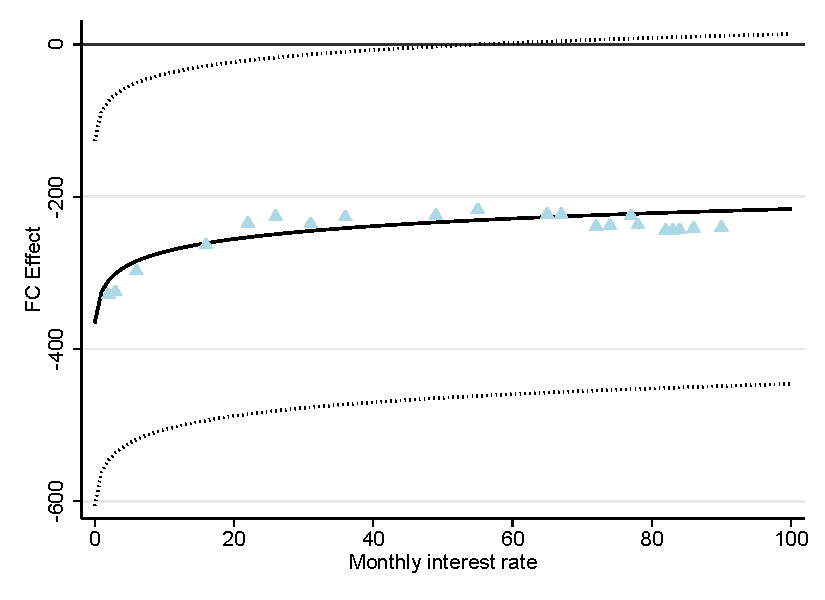
\includegraphics[width=0.45\textwidth]{Figuras/discount_effect.pdf}
    \end{center}
\end{figure}   
    \begin{itemize}
    \item   Commitment contract imposes up-front costs for later benefits (collateral recovery).  
    \item Can impatience explain why not take up a contract that decreases overall cost?
    \item  Requires a rate of ~2,000\% to make NPV cost effect insignificant. 
    \end{itemize}
}

\only<2>{  
  
    \begin{itemize}
    \item   Standard behavioral angle:  compliers are sophisticated time-consistent, non-compliers are a mix of naifs and the time consistent (who don't need commitment).  
    \item We have survey measure of time inconsistency taken at baseline.
    \item  Effect of Forcing should be entirely among the time-inconsistent.  Is this true? 
    \end{itemize}
}

\only<3>{  
  
    \begin{itemize}
    \item   Asked question prior to assignment, borrowing about subjective probability of recovering.  
    \item Mean of prior prediction is XX\%, true recovery in control is YY\%.
    \item  Use prediction of default in control, subjective priors to measure overconfidence.  Does this explain large TUT? 
    \end{itemize}
}
\end{frame}




\begin{frame}{Paternalism and learning}
    

    \begin{itemize}
    \item   Are those with a greater experience of pawning less over-confident?  
    \begin{itemize}
        \item Observational analysis of overconfidence by number of prior pawns.
    \end{itemize}  
    \item   Do people learn from Forced exposure to the program that they benefit from it?  
    \begin{itemize}
        \item Subsequent to the experimental loan, those exposed to different treatments returned to branches where they were offered Choice.  What did they do?
    \end{itemize}  

    \end{itemize}     

    
\end{frame}




\begin{frame}{Winners and losers:  Bounding}
    \begin{itemize}
        \item Bounding exercise
    \end{itemize}  

\end{frame}


\begin{frame}{Winners and losers:  Conditional TUTs}
     \begin{itemize}
        \item Conditional TUTs
    \end{itemize}  
 
\end{frame}



\section{Conclusion}
\begin{frame}{Conclusion}
    \begin{itemize}
        \item Results suggest selection on gains, but still large effects of imposing commitment on non-compliers.
        \item  Default-inclusive APR falls from XX\% in the Control to YY\% in the Forced arm
        \item Mystery of low takeup combined with large TUT seems best explained by over-confidence among pawnshop customers.
        \item  This is a market where lenders profit from default.  If competitive, interest rates would have to rise to compensate for improved repayment.  Holding demand and repayment fixed, current 75\% would have to rise to XX\%.  Welfare transfer from repayers in the control state to those who are helped to repay by commitment.
        \item Laibson has spoken of `veiled paternalism' in contexts where principals desire reliability; here we have a case of `veiled non-paternalism' where features encouraging default are embedded.
        \item Suggests mandated commitment-based contract structures in payday/pawnshop loans as a form of pro-poor regulation?
    \end{itemize}  
\end{frame}

\appendix

\section{Appendix}


\begin{frame}{Difference number in pawns}
    \[Pawns \: per \: day_{jt} = \alpha_j + \gamma f(t) + \beta_b \mathbbm{1}(t \in MB)_{t} +\beta_a \mathbbm{1}(t \in MA)_{t}\]
    
    \begin{table}[H]
\caption{Number of pawns balance before and after the experiment}
\label{num_pawns_bal}
\begin{center}
\scriptsize{% Table generated by Excel2LaTeX from sheet 'num_pawns_bal'
\begin{tabular}{lcccc}
\toprule
      & \multicolumn{4}{c}{Pawns per day} \\
\midrule
      & 0-degree & 1-degree & 2-degree & 3-degree \\
\midrule
\midrule
      & (1)   & (2)   & (3)   & (4) \\
\midrule
\midrule
$\beta_a$ & 2.48  & -3.32 & -0.65 & -0.65 \\
      & (1.36) & (1.85) & (2.80) & (2.80) \\
$\beta_b$ & 0.20  & 1.82  & 1.32  & 1.32 \\
      & (0.97) & (0.93) & (0.67) & (0.67) \\
      &       &       &       &  \\
\midrule
Observations & 628   & 628   & 628   & 628 \\
R-sq  & 0.737 & 0.747 & 0.747 & 0.747 \\
Branch FE & \checkmark & \checkmark & \checkmark & \checkmark \\
\bottomrule
\bottomrule
\end{tabular}%
}
\end{center}
\end{table}
\end{frame}


\begin{frame}{Balance and Summary statistics}
    \begin{table}[H]
\caption{Summary statistics and Balance}
\label{SS}
\begin{center}
\resizebox{.65\textwidth}{!}{
\scriptsize{% Table generated by Excel2LaTeX from sheet 'SS'
\begin{tabular}{lcccccccc}
\toprule
      &       &       & \multicolumn{5}{c}{Treatment arms}    &  \\
\midrule
      &       &       &       & \multicolumn{2}{c}{No Choice } & \multicolumn{2}{c}{Choice} &  \\
\midrule
\midrule
      & Overall & Pre-experiment & Control & Fee   & Promise & Fee   & Promise & p-value \\
\midrule
      & \multicolumn{8}{c}{Panel A : Administrative Data} \\
\midrule
\midrule
Loan amount  & 2197  & 2239  & 2301  & 2147  & 2133  & 2181  & 2089  & 0.32 \\
      & (25)  & (39)  & (79)  & (72)  & (74)  & (65)  & (65)  &  \\
Monday & 0.18  & 0.16  & 0.18  & 0.16  & 0.17  & 0.19  & 0.21  & 0.96 \\
      & (0.02) & (0.03) & (0.05) & (0.05) & (0.06) & (0.06) & (0.05) &  \\
Number of branch-day pawns & 34    & 36    & 31    & 31    & 32    & 37    & 34    & 0.38 \\
      & (0.82) & (1.25) & (2.2) & (2.35) & (2.38) & (2.65) & (1.76) &  \\
\midrule
Number of branch-days & -     &       & 84    & 80    & 68    & 93    & 82    &  \\
Obs   & 21808 & 8366  & 2601  & 2484  & 2156  & 3435  & 2766  &  \\
\midrule
      & \multicolumn{8}{c}{Panel B : Survey Data (conditional on pawning)} \\
\midrule
\midrule
Woman & 0.73  &       & 0.76  & 0.72  & 0.73  & 0.72  & 0.74  & 0.41 \\
      & (0.01) &       & (0.02) & (0.02) & (0.02) & (0.02) & (0.01) &  \\
Age   & 43.31 &       & 43.16 & 43.17 & 42.96 & 43.96 & 43.06 & 0.79 \\
      & (0.28) &       & (0.57) & (0.79) & (0.65) & (0.61) & (0.52) &  \\
Subjective value & 3068  &       & 3151  & 2978  & 2985  & 3114  & 3079  & 0.41 \\
      & (39)  &       & (69)  & (91)  & (76)  & (85)  & (100) &  \\
Has pawn before & 0.9   &       & 0.89  & 0.9   & 0.89  & 0.91  & 0.89  & 0.68 \\
      & (0)   &       & (0.01) & (0.01) & (0.01) & (0.01) & (0.01) &  \\
Subj. pr. of recovery & 93.14 &       & 92.74 & 92.16 & 93.6  & 93.67 & 93.3  & 0.46 \\
      & (0)   &       & (0.55) & (0.86) & (0.6) & (0.47) & (0.6) &  \\
+High-school & 0.66  &       & 0.66  & 0.67  & 0.65  & 0.67  & 0.64  & 0.74 \\
      & (0.01) &       & (0.02) & (0.02) & (0.02) & (0.02) & (0.02) &  \\
Survey response rate & 0.78  &       & 0.77  & 0.75  & 0.8   & 0.77  & 0.79  & 0.5 \\
      & (0.01) &       & (0.02) & (0.03) & (0.02) & (0.02) & (0.02) &  \\
\midrule
Obs   & 10431 &       & 2000  & 1855  & 1732  & 2652  & 2192  &  \\
\midrule
\midrule
      & \multicolumn{8}{c}{Panel C : Survey Data (unconditional)} \\
\midrule
\midrule
Woman & 0.74  & 0.75  & 0.76  & 0.72  & 0.73  & 0.72  & 0.74  & 0.32 \\
      & (0.01) & (0.01) & (0.02) & (0.02) & (0.02) & (0.02) & (0.01) &  \\
Age   & 43.24 & 43.06 & 43.2  & 43.21 & 43.01 & 44.07 & 43.07 & 0.79 \\
      & (0.21) & (0.32) & (0.56) & (0.77) & (0.66) & (0.61) & (0.51) &  \\
Subjective value & 3112  & 3192  & 3145  & 2985  & 3010  & 3111  & 3082  & 0.41 \\
      & (36)  & (75)  & (68)  & (88)  & (76)  & (84)  & (99)  &  \\
Has pawn before & 0.89  & 0.88  & 0.89  & 0.9   & 0.89  & 0.91  & 0.89  & 0.56 \\
      & (0.01) & (0.01) & (0.01) & (0.01) & (0.01) & (0.01) & (0.01) &  \\
Subj. pr. of recovery & 92.64 & 91.84 & 92.73 & 92.19 & 93.66 & 93.71 & 93.34 & 0 \\
      & (0.2) & (0.31) & (0.54) & (0.84) & (0.59) & (0.46) & (0.59) &  \\
+High-school & 0.63  & 0.6   & 0.66  & 0.67  & 0.65  & 0.66  & 0.64  & 0.01 \\
      & (0.01) & (0.01) & (0.02) & (0.02) & (0.02) & (0.02) & (0.02) &  \\
\% ended up pawning &       &       & 0.98  & 0.97  & 0.99  & 0.98  & 0.99  & 0.25 \\
\midrule
Obs   & 17546 & 6919  & 2035  & 1907  & 1757  & 2710  & 2218  &  \\
\bottomrule
\bottomrule
\end{tabular}%
}
}
\end{center}

%\textit{Do file: } \texttt{ss\_att.do}
\end{table}
\end{frame}


\begin{frame}{Histogram of payments}

\begin{columns}
\begin{column}{.33\textwidth}
    \begin{figure}[H]
    \caption{Status-quo}
    \begin{center}
        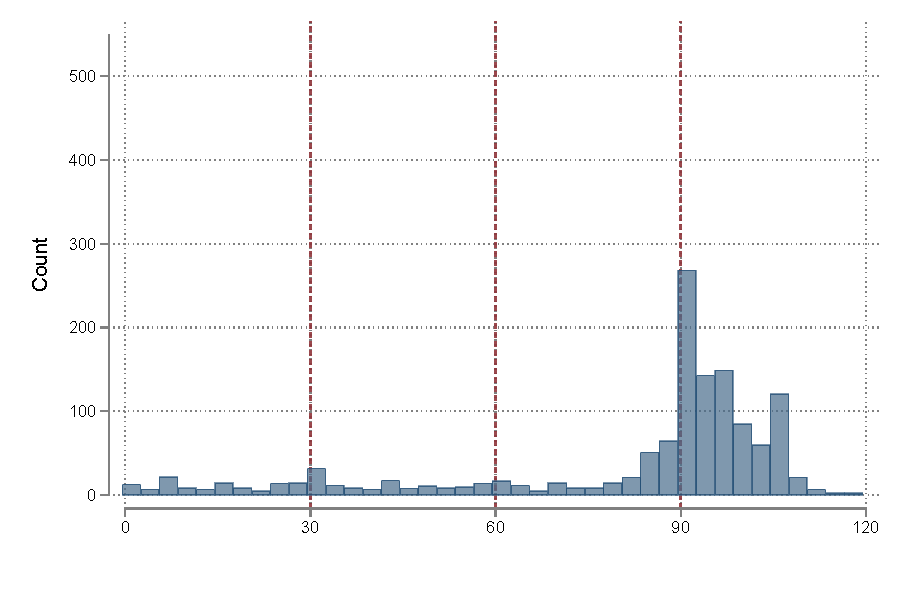
\includegraphics[width=\textwidth]{Figuras/hist_payments_sq.pdf}
    \end{center}
\end{figure}
\end{column}

\begin{column}{.33\textwidth}
    \begin{figure}[H]
    \caption{Forced commitment}
    \begin{center}
        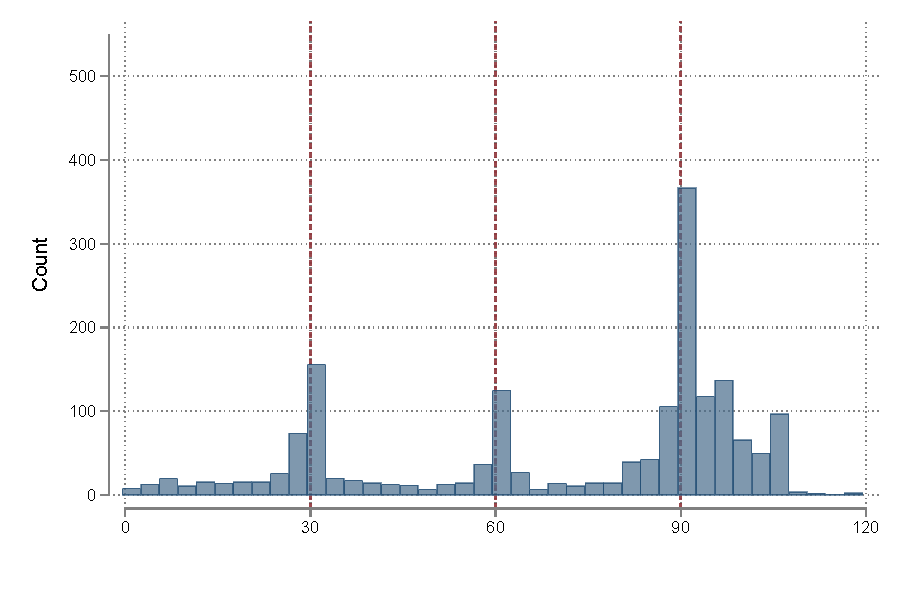
\includegraphics[width=\textwidth]{Figuras/hist_payments_fc.pdf}
    \end{center}
\end{figure}
\end{column}

\begin{column}{.33\textwidth}
    \begin{figure}[H]
    \caption{Choice commitment}
    \begin{center}
        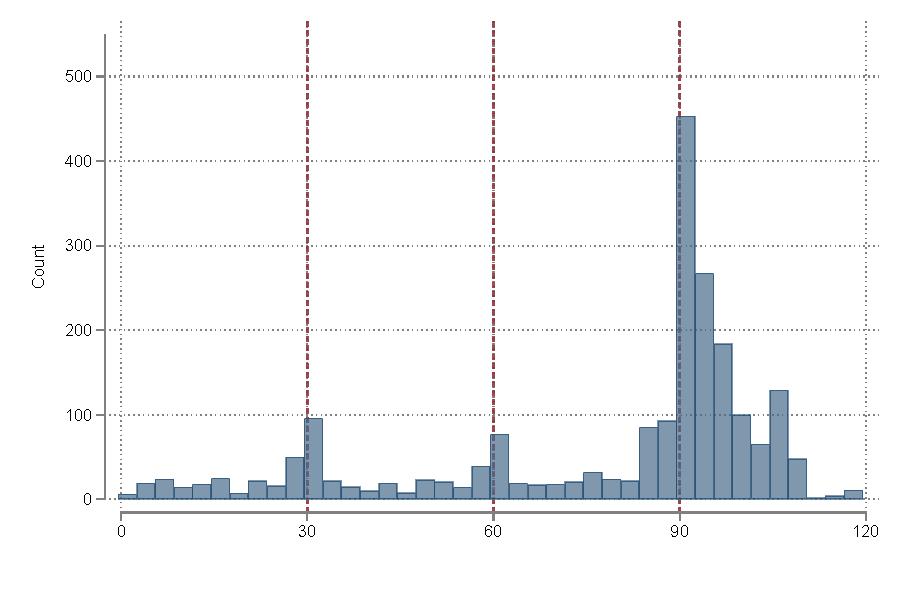
\includegraphics[width=\textwidth]{Figuras/hist_payments_cc.pdf}
    \end{center}
\end{figure}
\end{column}
\end{columns}

\end{frame}

\begin{frame}{Several definitions of cost}

\begin{table}[H]
\caption{Effects on several definitions of cost}
\label{table_robustness_fc}
\begin{center}
\resizebox{0.95\textwidth}{!}{
\scriptsize{% Table generated by Excel2LaTeX from sheet 'fc_robustness'
\begin{tabular}{lccccc}
\toprule
      & FC    & FC (subj.value) & FC +  tc & FC - interest & FC (subj.value) + tc - int \\
\midrule
      & (1)   & (2)   & (3)   & (4)   & (5) \\
\midrule
\midrule
Forced commitment & -204.0*** & -299.9*** & -207.7*** & -98.5*** & -146.3** \\
      & (48.1) & (83.3) & (49.0) & (36.7) & (72.8) \\
Choice comitment & -38.9 & -56.4 & -32.6 & -30.7 & -25.3 \\
      & (49.8) & (83.5) & (50.9) & (39.2) & (74.4) \\
      &       &       &       &       &  \\
\midrule
Observations & 6304  & 6304  & 6304  & 6304  & 6304 \\
R-squared & 0.013 & 0.009 & 0.014 & 0.005 & 0.006 \\
Control Mean & 942.4 & 1389.9 & 1026.1 & 480.7 & 927.7 \\
\midrule
\midrule
      &       &       &       &       &  \\
\midrule
      & APR   & APR (subj.value) & APR +  tc & APR - interest & APR (subj.value) + tc - int \\
\midrule
      & (6)   & (7)   & (8)   & (9)   & (10) \\
\midrule
\midrule
Forced commitment & -0.11*** & -0.22*** & -0.13*** & -0.062*** & -0.097** \\
      & (0.019) & (0.051) & (0.028) & (0.019) & (0.044) \\
Choice comitment & -0.0086 & -0.053 & -0.0035 & -0.031* & -0.043 \\
      & (0.019) & (0.045) & (0.028) & (0.018) & (0.040) \\
      &       &       &       &       &  \\
\midrule
Observations & 6304  & 6304  & 6304  & 6304  & 6304 \\
R-squared & 0.031 & 0.011 & 0.027 & 0.008 & 0.007 \\
Control Mean & 0.57  & 1.12  & 0.72  & 0.31  & 0.84 \\
\bottomrule
\bottomrule
\end{tabular}%
}
}
\end{center}
 \scriptsize 
 
%\textit{Do file: } \texttt{fc\_robustness.do}
\end{table}
    
\end{frame}


\begin{frame}{Contract terms}

\begin{figure}[H]
     \caption{Contract Terms Summary}
    \label{PaperSlip}
    \begin{center}
        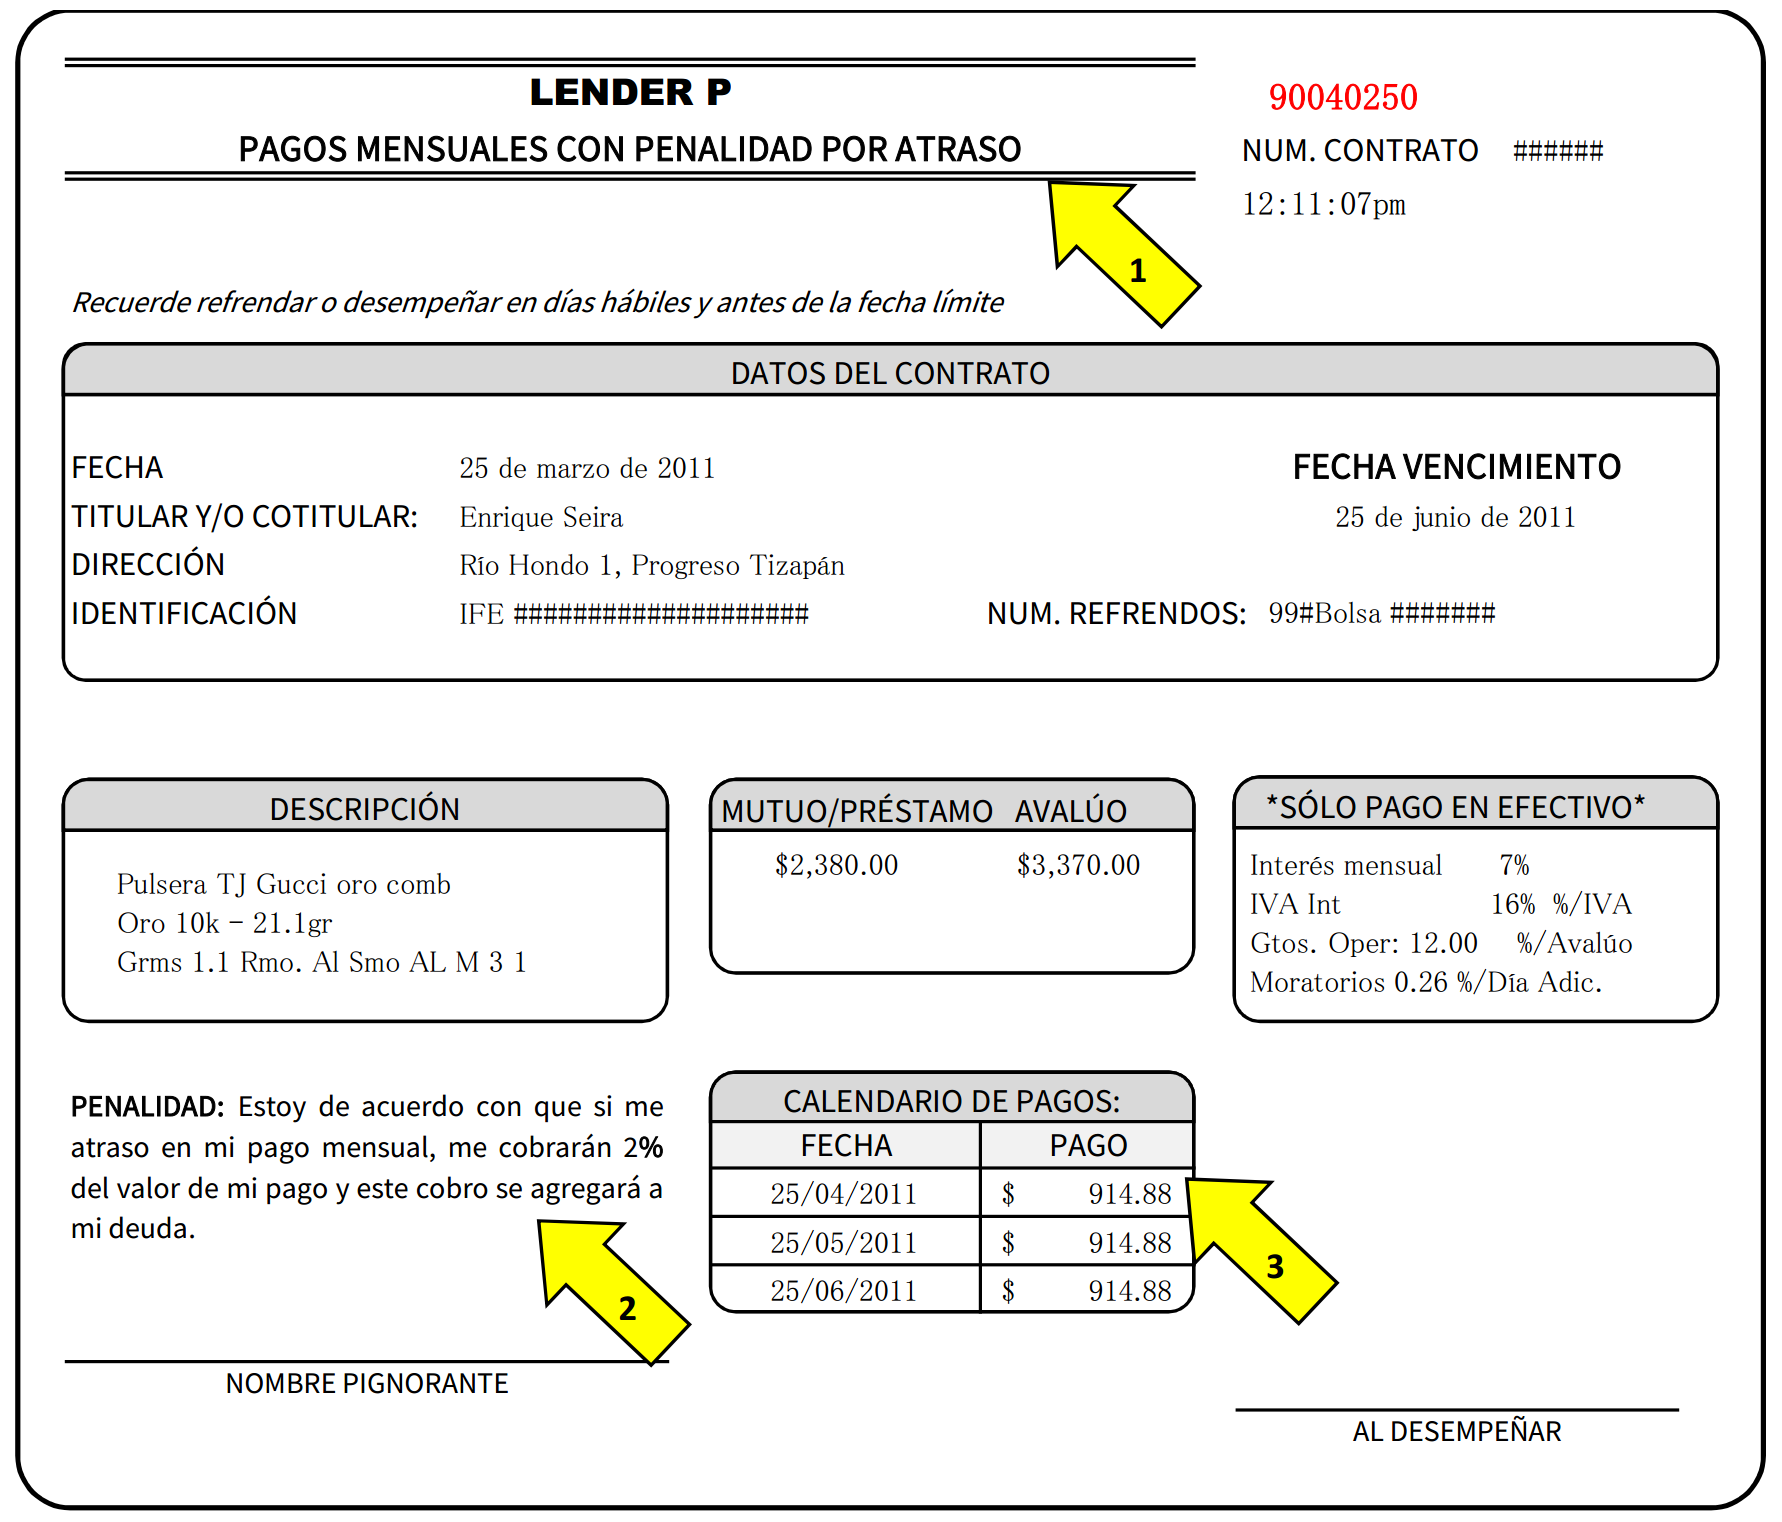
\includegraphics[width=0.65\textwidth]{Figuras/TicketLenderP.png}

    \end{center}

\end{figure}





\end{frame}

\begin{frame}{Explanatory material}
    \begin{figure}[H]
     \caption{Explanatory Material}
    \label{ExplanatoryMaterial}
    \begin{center}
        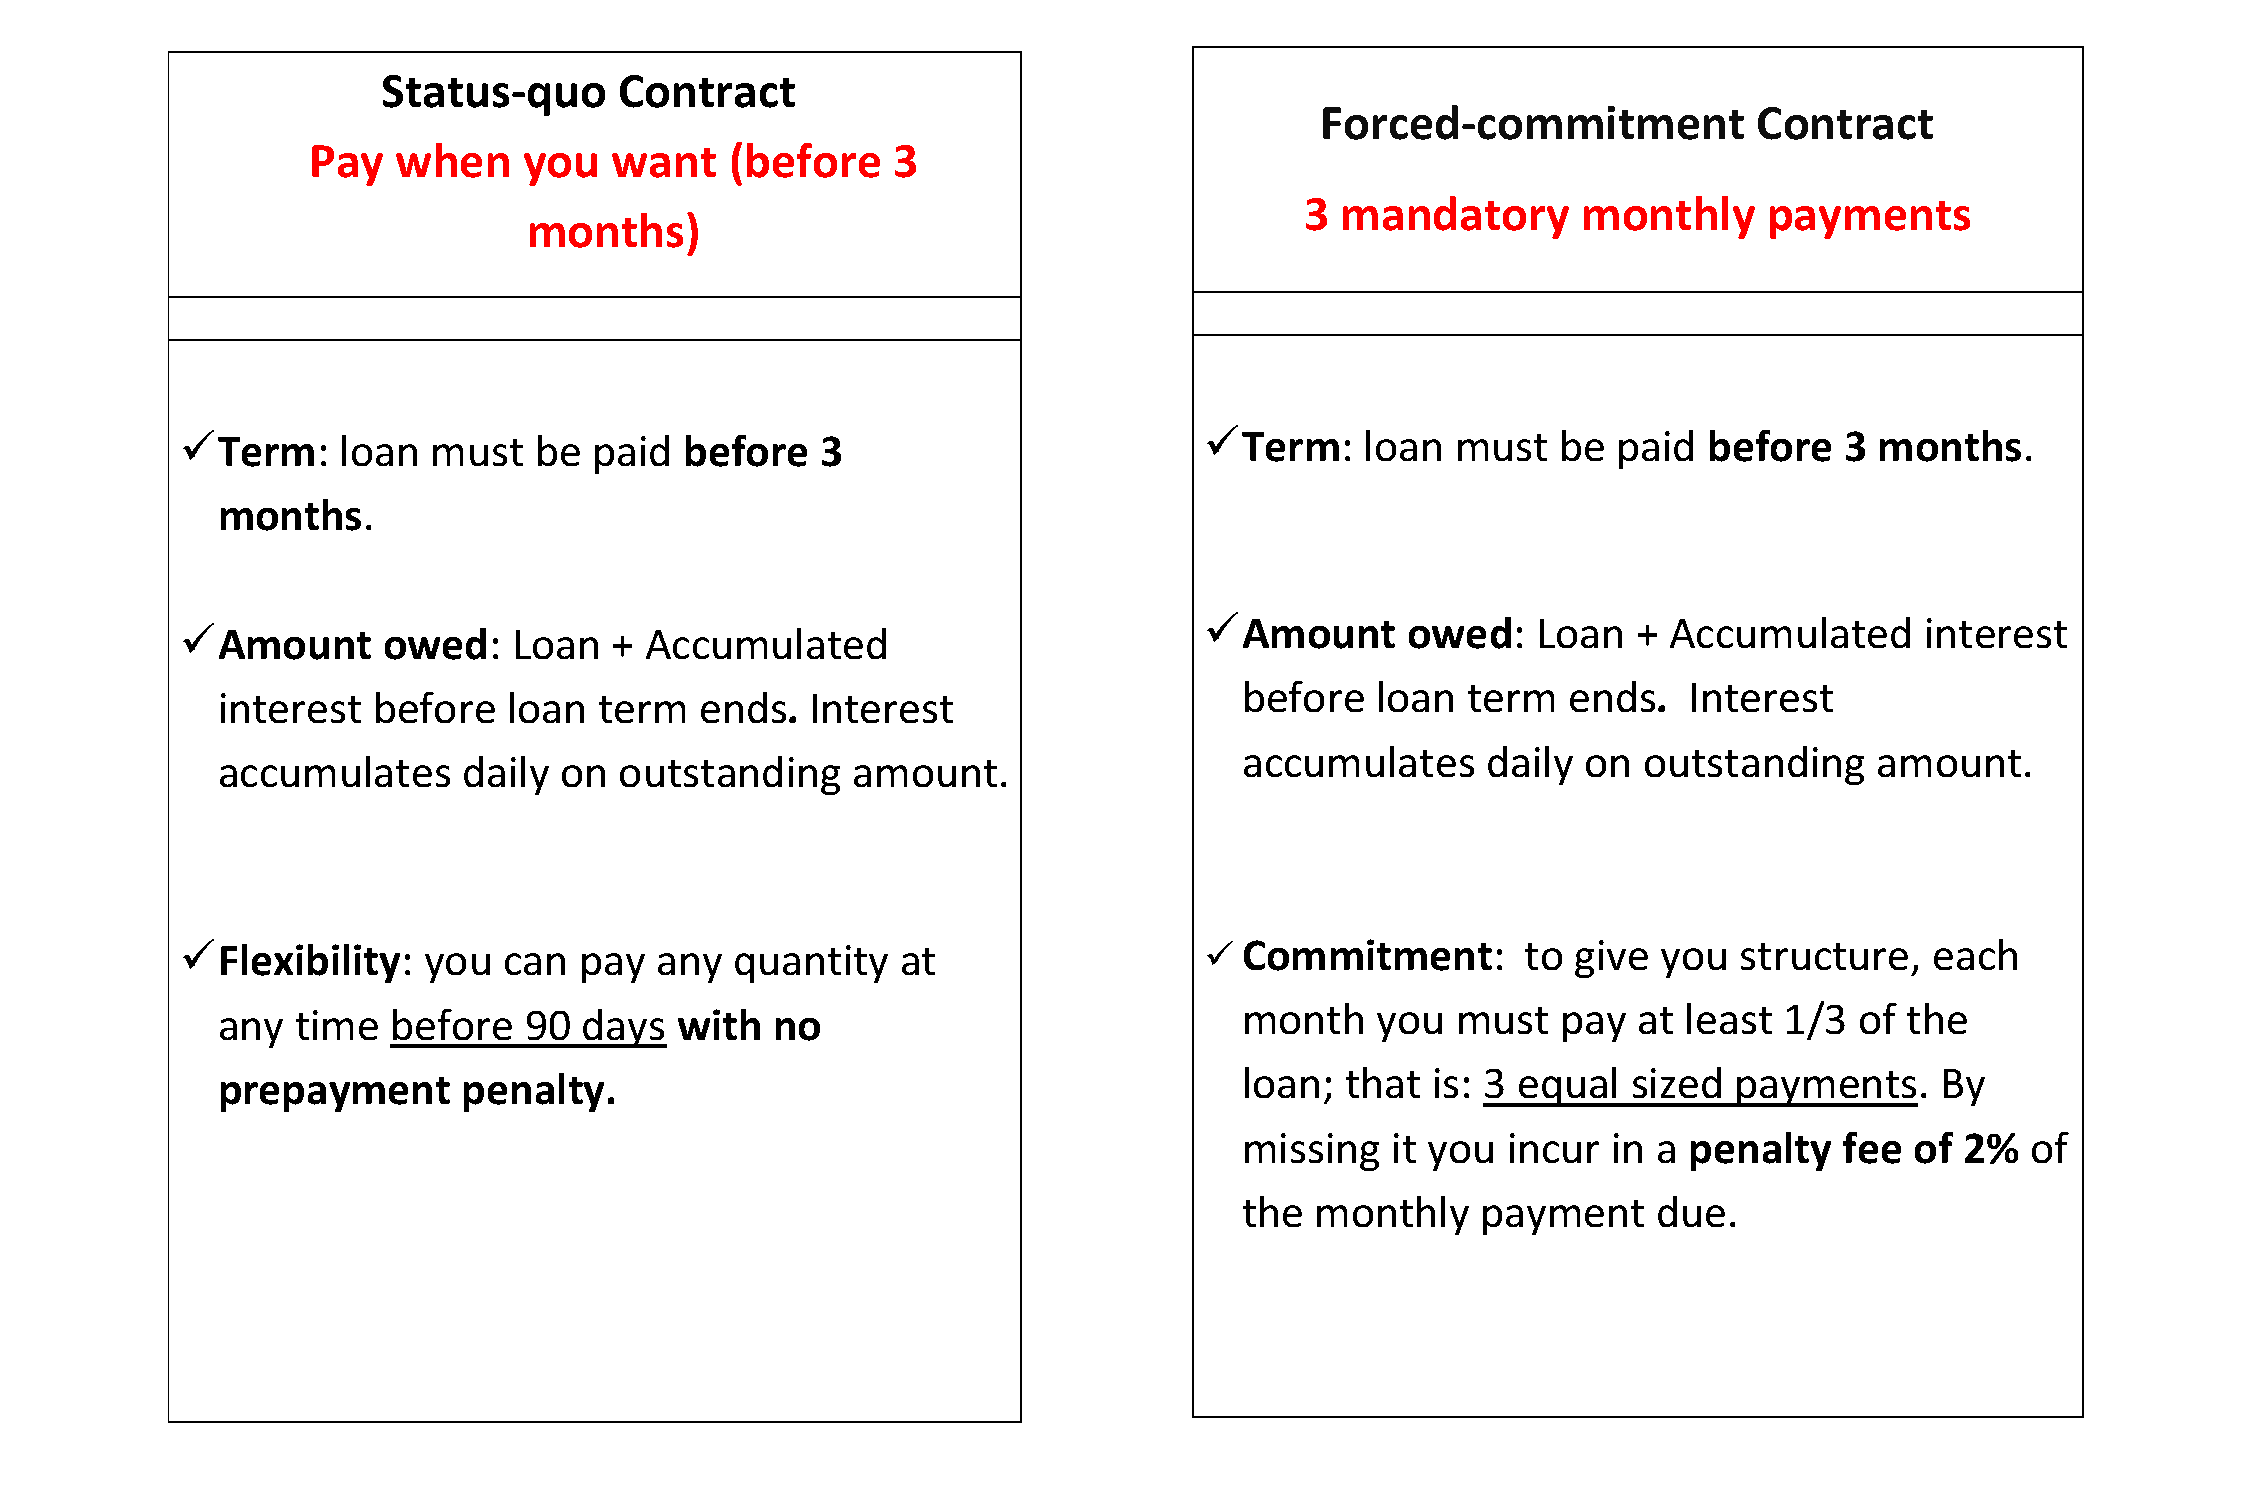
\includegraphics[width=0.9\textwidth]{Figuras/micas.pdf}
    \end{center}
\end{figure}
\end{frame}

\begin{frame}{Survival Graph}
 
\begin{figure}[H]
        \caption{Recovery}
    \label{survival_graph}
    \begin{center}
        \centering
        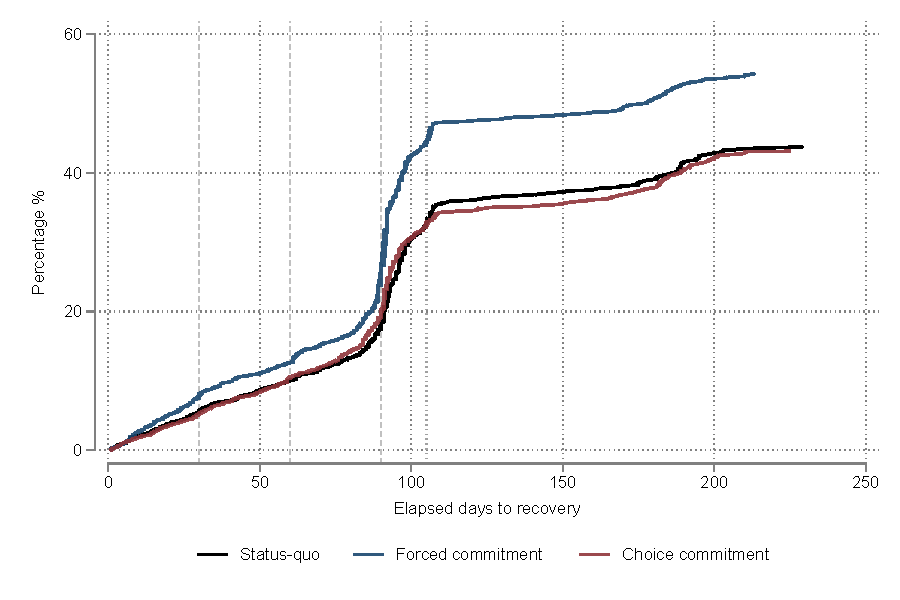
\includegraphics[width=0.75\textwidth]{Figuras/survival_graph_unpledge.pdf}
    \end{center}
\end{figure}   
\end{frame}

\begin{frame}{Interpolation on bounding censoring}
    
\begin{figure}[H]
        \caption{Significance area for Default}
    \label{interpolation_censoring_imp}
    \begin{center}
        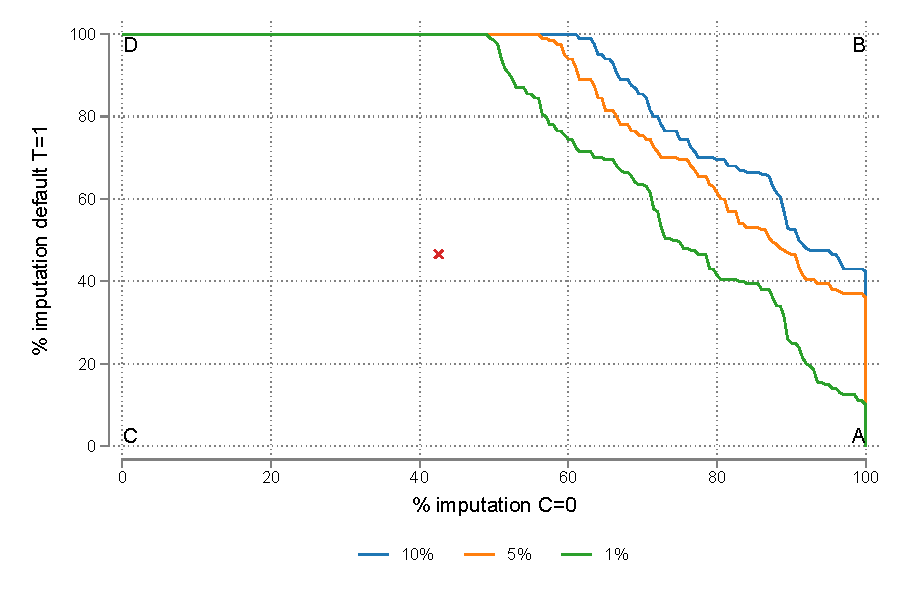
\includegraphics[width=0.75\textwidth]{Figuras/frontera_sig_def_imp.pdf}
    \end{center}
\end{figure}
\end{frame}


\begin{frame}{Bounding Individual Treatment Effects}
\label{fan_park_bounds}    

\begin{figure}[H]
    \caption{Fan \& Park bounds for benefit in APR\% }
    
    \begin{center}
        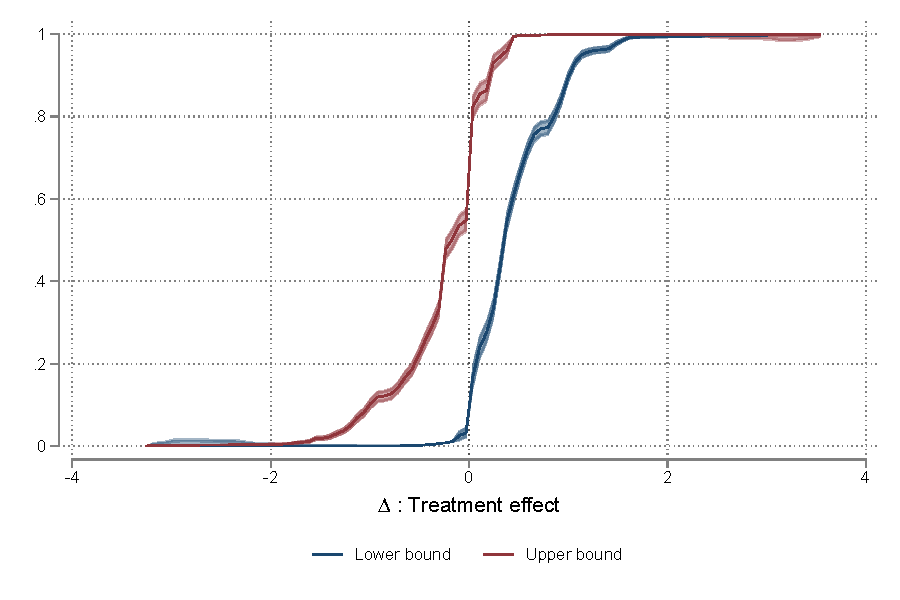
\includegraphics[width=0.75\textwidth]{Figuras/fan_park_bounds_apr.pdf}
    \end{center}
   
\end{figure}
 \hyperlink{choice_hte}{\beamerbutton{Back}}
\end{frame}

\begin{frame}{Identification of treatment parameters}
\label{identification_randomized_choice}
\begin{equation*}
    Y_i = \mathbbm{1}(Z_i =0) Y_{i0} + \mathbbm{1}(Z_i = 1)  Y_{i1}  + \mathbbm{1}(Z_i = 2) \left[(1 - C_i) Y_{i0} + C_i Y_{i1} \right].
\label{eq:potentialOutcomes}
\end{equation*}

    Viewing $Z_i$ as an instrumental variable, the randomized choice design can be interpreted as a \emph{pair} of RCTs, each subject to one-sided non-compliance. \\
    \begin{itemize}
        \item The first of these compares $Z_i=0$ to $Z_i = 2$.  This setting is identical to a ``randomized encouragement'' design in which treatment is only available to those who are encouraged: $Z_i = 2$. Under this interpretation, those with $C_i = 1$ are ``the compliers'' and it follows that 
\begin{equation*}
\frac{\mathbbm{E}(Y_i|Z_i=2) - \mathbbm{E}(Y_i|Z_i =0)}{\mathbbm{E}(D_i|Z_i=2)-\mathbbm{E}(D_i|Z_i=0)}  = \mathbbm{E}(Y_{i1} - Y_{i0}|C_i = 1)
\label{eq:ToT}
\end{equation*}

\item The second considers $Z_i = 1$ to be the ``encouragement'' and compare the outcomes for these individuals to those with $Z_i = 2$.
\begin{equation*}
\frac{\mathbbm{E}(Y_i|Z_i=1) - \mathbbm{E}(Y_i|Z_i =2)}{\mathbbm{E}(D_i|Z_i=1)-\mathbbm{E}(D_i|Z_i=2)}  = \mathbbm{E}(Y_{i1} - Y_{i0} | C_i = 0)
\label{eq:TuT}
\end{equation*}
    \end{itemize}

\hyperlink{rc_design}{\beamerbutton{Back}}


\end{frame}

\end{document}










\begin{figure}[H]
    \caption{Choice of contracts and treatment effects (ToT \& TuT)}
    \label{choose_wrong}
    \begin{center}
        \begin{subfigure}{0.45\textwidth}
        \caption{Mistakes in choice arm}
        \centering
        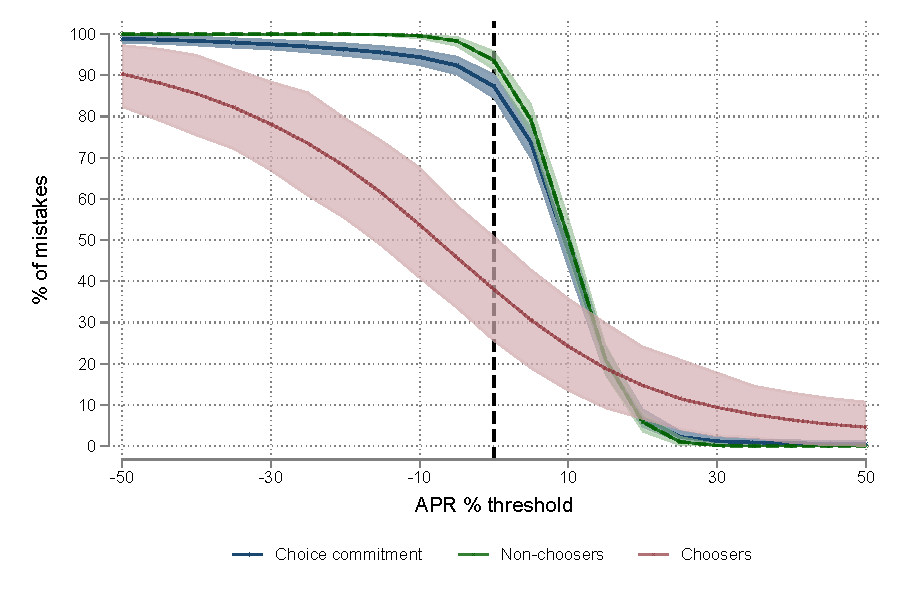
\includegraphics[width=\textwidth]{Figuras/line_cw_apr_tot_tut.pdf}
        
    \end{subfigure}
        \begin{subfigure}{0.45\textwidth}
        \caption{Financial value of mistake}
        \centering
        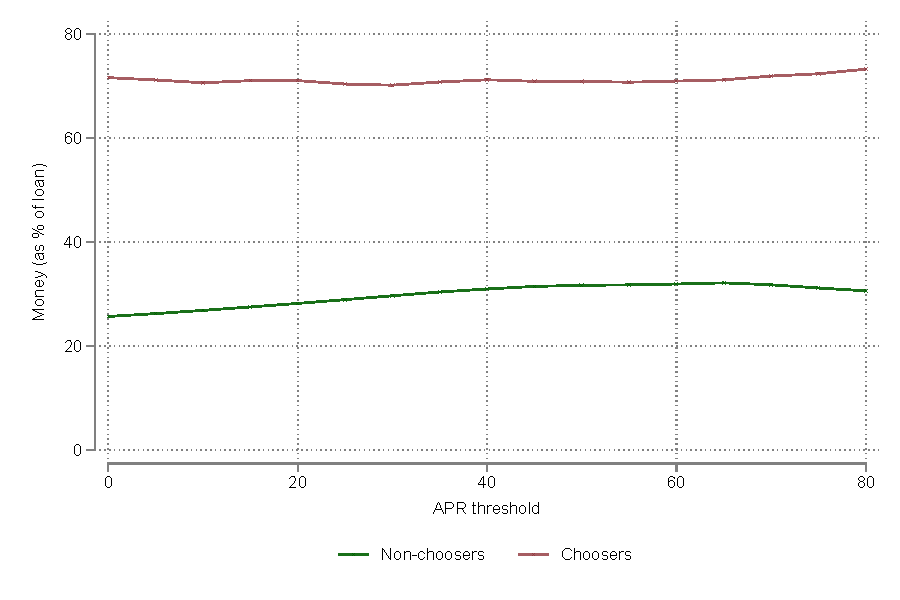
\includegraphics[width=\textwidth]{Figuras/money_cw_apr_tot_tut.pdf}

    \bigskip
        
    \end{subfigure}
        \begin{subfigure}{0.45\textwidth}
        \caption{\% better when forced to forced commitment}
        \centering
        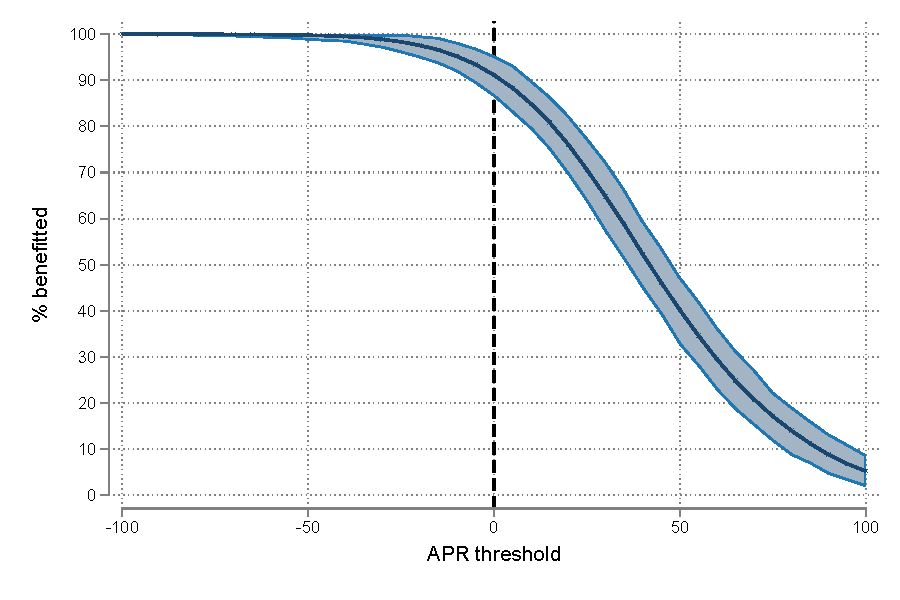
\includegraphics[width=\textwidth]{Figuras/line_better_forceall_apr_te_cf.pdf}
        
    \end{subfigure}
    
    \end{center}
\end{figure}



